\chapter{Scientific motivation}
\label{ch:scientific_motivation}

Our understanding of the universe is constantly evolving, and the few-hundred-year rise of scientific experimentation and reasoning has propelled us towards an increasingly sophisticated and elegant theory of the cosmos and its history. While there are many ways to probe the universe's evolution---including mapping planet orbits, dissecting the characteristics and life cycles of stars, inspecting the motion of galaxies, and analyzing interstellar dust---the field of cosmology, or the study of the universe on its largest scales, has emerged as a cornerstone of modern physics.

The prevailing theory of modern cosmology is the so-called $\Lambda$CDM model, which states that the universe is composed of dark energy---quantified by the cosmological constant $\Lambda$---and cold dark matter (CDM), in addition to the more familiar baryonic matter and radiation energy. $\Lambda$CDM asserts that the universe expanded from a dense, hot plasma into the isotropic, homogeneous, cosmic web of galaxy clusters in which we exist today.

Despite $\Lambda$CDM's success, it has several including the so-called Horizon, Flatness, and Magnetic Monopole problems. These issues\footnote{In addition, $\Lambda$CDM does not describe the particle nature of dark matter or dark energy, which are active areas of particle physics research.} are solved by the theoretic paradigm of \textit{inflation}, which predicts a period of super-luminal expansion $\sim$~$10^{-36}$~s after the birth of the universe at $t = 0$. While inflation elegantly describes many observed cosmological phenomenon, it is is not yet experimentally verified. 

The cosmic microwave background (CMB) is radiation remnant of the hot Big Bang, and since their discovery in ~blah, CMB spatial intensity fluctuations have been one of the most powerful tools to constrain the universe's composition and history. Inflation, if true, would have left a unique signature on the polarization of the CMB, driving observatories to improve polarization sensitivity in an effort to detect inflation, in addition to better constraining $\Lambda$CDM. As instrumental sensitivity improves, the hypothesized inflation-generated CMB polarization signal is becoming buried by galactic foregrounds, necessitating not only an exquisite measurement of the CMB but also of the spatial and spectral characteristic of interstellar dust and synchrotron radiation. Therefore, the research area of CMB cosmology is pushing to improve both statistical and systematic sensitivity by building bigger, more precise telescopes with increasing throughput and detector counts.

In this chapter, we review our state-of-the-art understanding of cosmology, introduce the cosmic microwave background, and pose the unanswered questions and challenges that researchers are tackling as I write.

%%%%%%%%%%%%%%%%%%%%%%%%%%%%%%%%
%%%%%%%%%%%%%%%%%%%%%%%%%%%%%%%%
%%%%%%%%%%%%%%%%%%%%%%%%%%%%%%%%

\section{Big Bang Cosmology}
\label{sec:big_bang_cosmology}

General relativity relates space-time curvature---parameterized by the Einstein tensor $G_{\mu \nu}$---to its energy composition---parameterized by the energy-momentum tensor $T_{\mu \nu}$---using the Einstein field equations
\begin{equation}
    G_{\mu \nu} + \Lambda g_{\mu \nu} = \frac{8 \pi G}{c^{4}} T_{\mu \nu} \, , 
    \label{eq:einstein_field_equations}
\end{equation}
where $g_{\mu \nu}$ is the metric tensor, $\Lambda$ is the \textit{cosmological constant}, $G$ is gravitational constant, $c$ is the speed of light. Under the assumptions of homogeneity and isotropy, or that there are no ``special'' places in the universe, the field equations are solved by the Friedmann-Robertson-Walker (FRW) metric, whose space-time invariant is defined in hyperspherical coordinates as
\begin{equation}
    \dd s^{2} = - \dd t^{2} + a^{2}(t) \left[ \dd r^{2} + S_{k}^{2}(r) \dd \Omega^{2} \right] \, .
    \label{eq:frw_metric}
\end{equation}
Here, $t$ is proper time, $a(t)$ is the \textit{scale factor}, $r$ is the radial coordinate, $\Omega$ is solid angle with Jacobian $\dd \Omega^{2} = \dd \theta^{2} + \sin^{2} \theta \dd \phi^{2}$, and
\begin{equation}
    S_{k}(r) \equiv \frac{\sin(\sqrt{k} r)}{\sqrt{k}} \, ,
    \label{eq:curvature}
\end{equation}
where $k$ can be thought of as the space-time curvature today. In the FRW metric, the scale factor $a(t)$ measures the expansion of space as a function of time, and therefore it's convenient to define the \textit{comoving distance}
\begin{equation}
    \chi \equiv \frac{r(t)}{a(t)} \, ,
    \label{eq:comoving_distance}
\end{equation}
which is constant in time. A depiction of the \textit{comoving grid} and its relationship to proper distance and the scale factor are shown in Figure~\ref{fig:comoving_grid}.

\begin{figure}[!t]
    \centering
    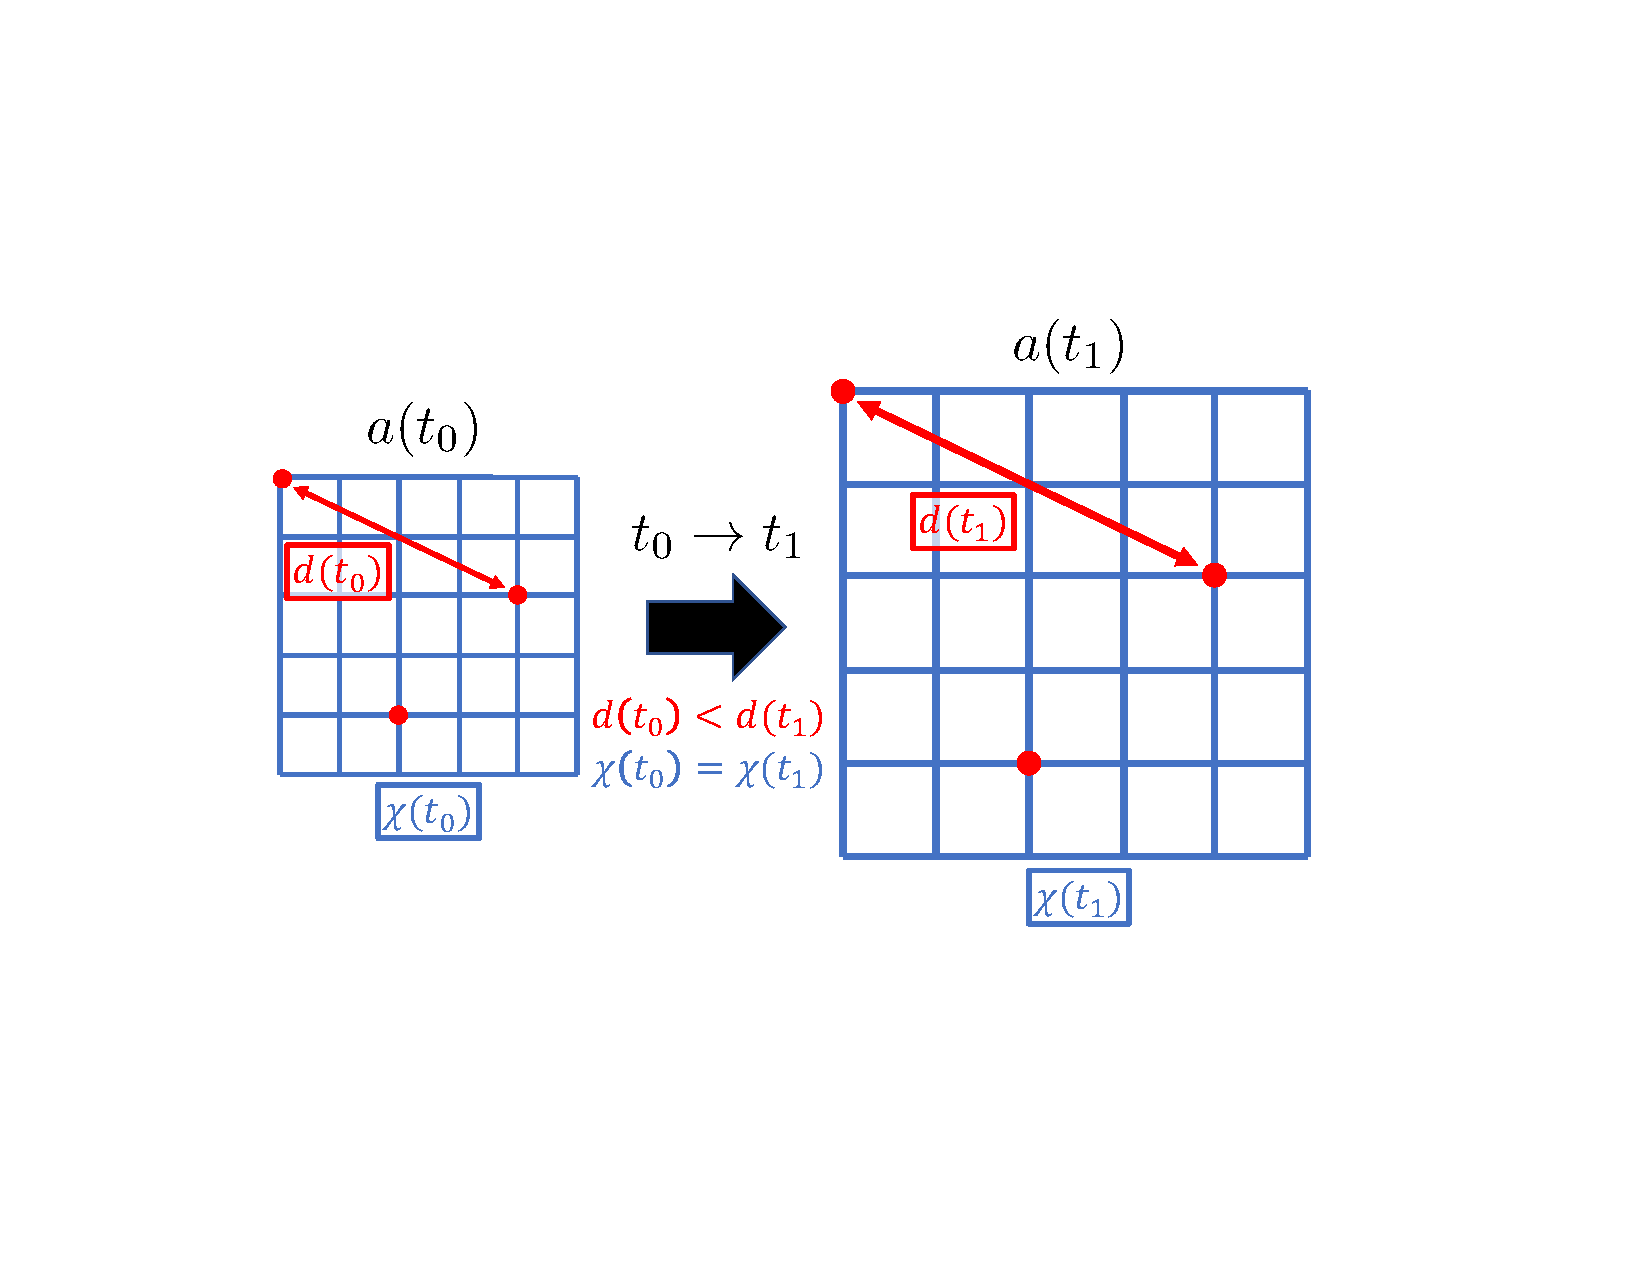
\includegraphics[width=0.9\linewidth, trim=3cm 5.5cm 3cm 5cm, clip]{ScientificMotivation/Figures/comoving_grid.pdf}
    \caption[A schematic of the comoving grid]{A schematic of the comoving grid. In the standard cosmological paradigm, the scale factor $a(t)$ grows with time, enlarging the distance between otherwise stationary objects, which are represented by red circles. However, in comoving coordinates, the distance between these objects remains constant.}
    \label{fig:comoving_grid}
\end{figure}

The solution Einstein's field equations given the FRW metric are
\begin{eqnarray}
    \left( \frac{\dot a}{a} \right)^{2} & = & \frac{8 \pi G}{3} \rho - \frac{k}{a^{2}} \\
    \frac{\ddot a}{a} & = & - \frac{4 \pi G}{3} \left( \rho + 3p \right) \, ,
    \label{eq:friedmann_equations}
\end{eqnarray}
where the overdots denote time derivatives, $\rho$ is energy density, and $p$ is isotropic pressure. These \textit{Friedman Equations} relate the universe's expansion history to that of its constituents and are the cornerstone of Big Bang cosmology. The expansion factor at present time is defined to be $a = 1$, and its time derivative is parameterized by the Hubble parameter
\begin{equation}
    H \equiv \frac{\dot a}{a} \, ,
    \label{eq:hubble_constant}
\end{equation}
which measures the rate at which space is expanding.

\begin{figure}
    \subfloat[\label{fig:hubble_diagram:a}]{
        \raisebox{1cm}{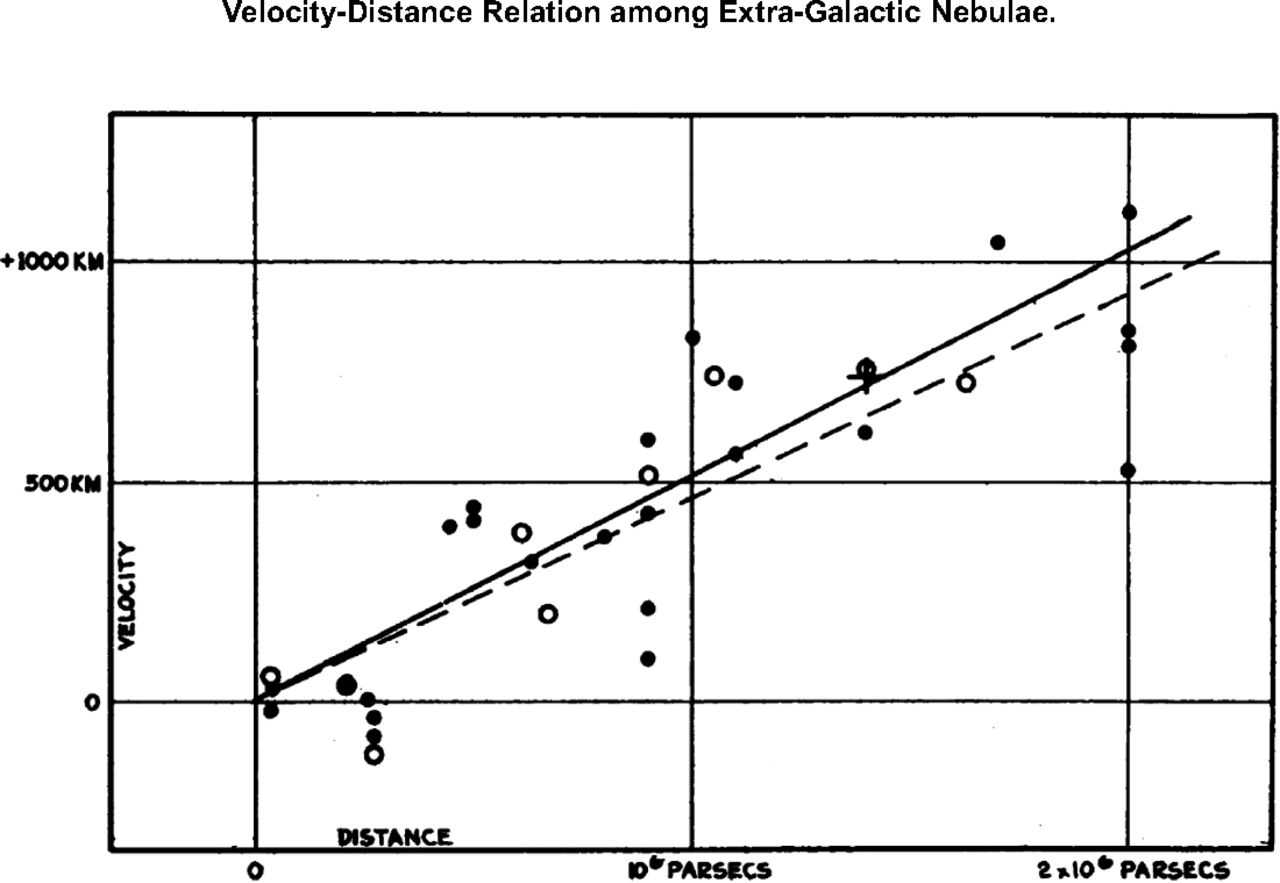
\includegraphics[width=0.48\linewidth]{ScientificMotivation/Figures/Hubble_redshiftRelation_1929.jpg}}
    }
    \subfloat[\label{fig:hubble_diagram:b}]{
        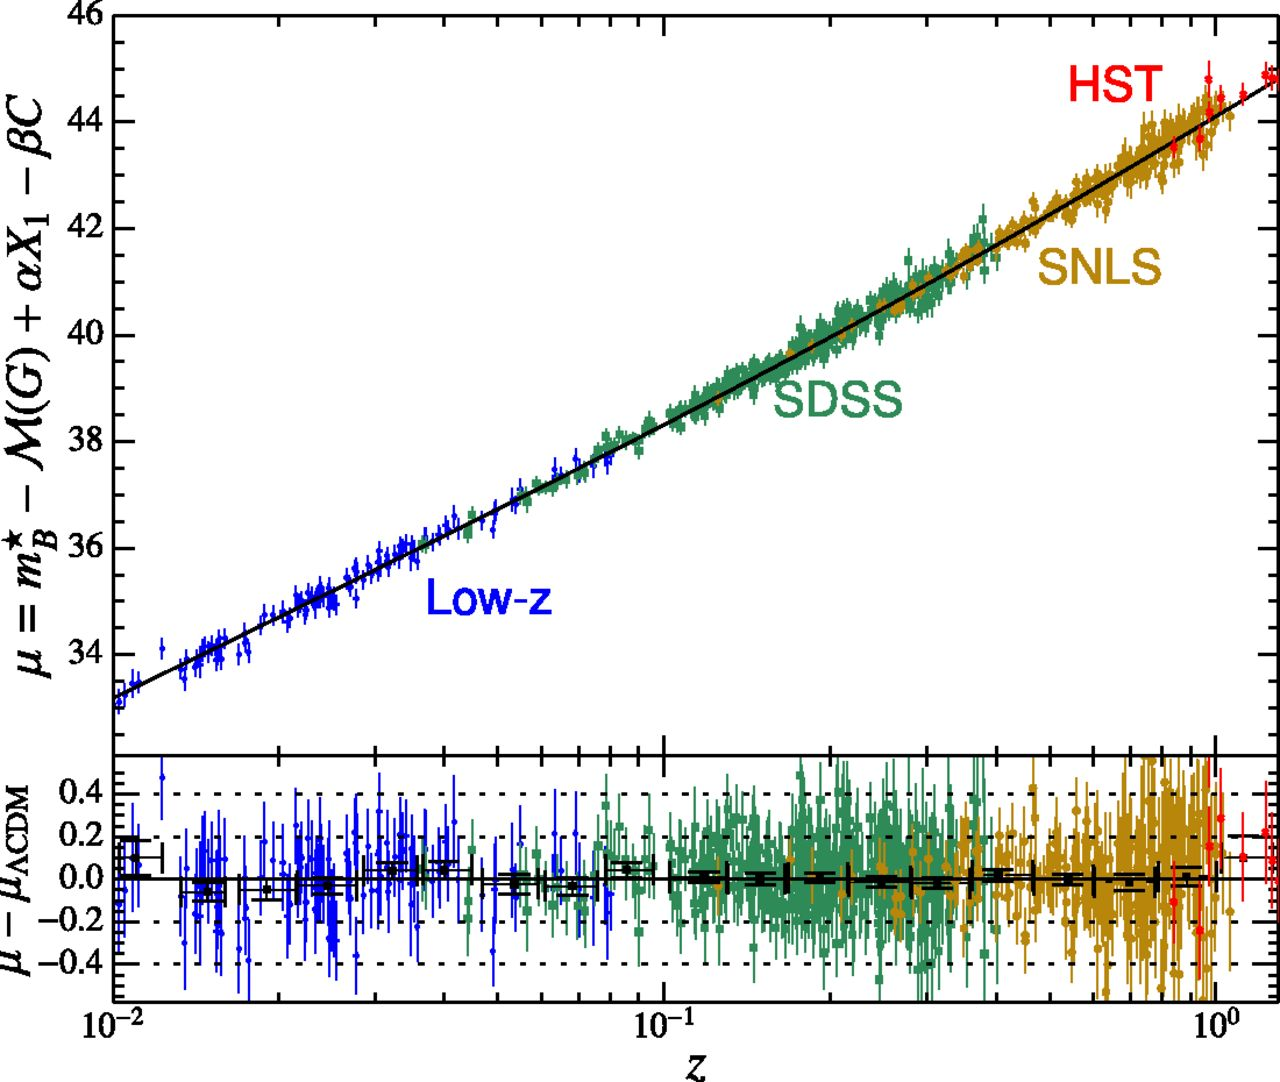
\includegraphics[width=0.48\linewidth]{ScientificMotivation/Figures/Bahcall_HubbleConstant_2015.jpg}
    }
    \caption[The original Hubble diagram and a modern version of it]{Two representations of the Redshift-velocity relationship, which is quantified by the Hubble constant. \ref{fig:hubble_diagram:a} shows Hubble's original diagram, published in 1929 \cite{hubble_relation_1929}. The filled circles and solid line show individual extra-galactic nebulae and distance-velocity relationship, respectively. The open circles and the dotted line show these nebulae grouped and fit. The clear trend demonstrates clearly that the universe is expanding. \ref{fig:hubble_diagram:b} shows a modern version of Hubble's plot, with collections of data from various experiments---Low-z, the Sloan Digital Sky Survey (SDSS), the Super Nova Legacy Survey, and the Hubble Space Telescope (HST)---which use supernovae to calibrate object distance \cite{bahcall_hubble_2015}.}
    \label{fig:hubble_diagram}
\end{figure}

The \textit{Hubble constant} $H_{0}$, or the current-time (a = 1) value of the Hubble parameter, was first measured by Edwin Hubble in 1929 using the redshift-distance relationship of extragalactic nebulae, as shown in Figure~\ref{fig:hubble_diagram:a}. Figure~\ref{fig:hubble_diagram:b} shows a a more modern measurement of $H_{0}$ from an assortment of telescopes and distant-ladder techniques, revealing a value of $H_{0} \approx 70$~km/s/MPc. While Hubble's measurement of turned out to be inaccurate, it was the first firm evidence for an expanding universe and birthed an era of precision cosmological measurements to characterize the dynamics of the universe on its largest scales.

We can conveniently rewrite the Friedmann equations in terms of the Hubble constant as
\begin{equation}
    H^{2} = H_{0}^{2} \left( \frac{\Omega_{r}}{a^{4}} + \frac{\Omega_{m}}{a^{3}} + \frac{\Omega_{k}}{a^{2}} + \Omega_{\Lambda} \right) \, ,
    \label{eq:friedmann_equation_densities}
\end{equation}
where $\Omega_{r}$, $\Omega_{m}$, $\Omega_{k}$, and $\Omega_{\Lambda}$ are the current-day densities of radiation, matter, curvature, and dark energy, respectively, with respect to the critical density
\begin{equation}
    \rho_{\mathrm{c}} = \frac{3}{8 \pi G} H_{0}^{2}\, .
    \label{eq:critical_density}
\end{equation}
The ratio of the actual density today to the critical density is given as $\Omega \equiv \rho_{0} / \rho_{\mathrm{c}}$ such that 
\begin{equation}
    \Omega = 1 + \frac{k}{H_{0}} \, ,
    \label{eq:total_density}
\end{equation}
The matter density $\Omega_{\mathrm{m}}$ includes that of dark matter, and the radiation density $\Omega_{\mathrm{r}}$ includes that of relativistic species. The best current estimates of the universe's constituents---most of which come from the Planck satellite mission---are shown in Table~\ref{tab:cosmological_parameters}. 

\begin{table}[]
    \centering
    \begin{tabular}{c|c}
         Parameter & Value \\
         \hline
         \hline
         $H_{0}$ & $67.66 \pm 0.42$ \\
         \hline
         $\Omega_{\mathrm{b}} h^{2}$ & $0.02242 \pm 0.00014$ \\
         \hline
         $\Omega_{\mathrm{c}} h^{2}$ & $0.14240 \pm 0.00087$ \\
         \hline
         $\Omega_{\mathrm{\Lambda}}$ & $0.6889 \pm 0.0056$ \\
         \hline
    \end{tabular}
    \caption{Cosmological parameters from Table~2 in the Planck 2018 publication. The error bars represent 68\% confidence limits, $\Omega_{\mathrm{k}} = 0$, as is true in a flat universe.}
    \label{tab:cosmological_parameters}
\end{table}

%%%%%%%%%%%%%%%%%%%%%%%%%%%%%%%%
%%%%%%%%%%%%%%%%%%%%%%%%%%%%%%%%
%%%%%%%%%%%%%%%%%%%%%%%%%%%%%%%%

\section{Cosmic microwave background}
\label{sec:cmb}

One of the most prominent predictions of the Big Bang model is the existence of a remnant background radiation. Because the universe is formed by the adiabatic expansion of space, at very early times, energy densities are very high, and therefore the universe's constituents---photons, electrons, positrons, protons, neutrons, and neutrinos---are in thermal equilibrium, forming what is often called the \textit{primordial plasma}. As the universe expands, its energy density dilutes (except for that of the cosmological constant) as in Equation~\ref{eq:friedmann_equation_densities}, and as the ``soup'' of particles cools, particles begin to decouple from the primordial plasma, or \textit{freeze out}. This process is called \textit{Big Bang Nucleosynthesis}, and it determines much of what we know about cosmic particle abundances today.

The ground-state binding energy of Hydrogen is 13.6~eV, and at temperatures substantially larger than this, ionizing radiation keeps Hydrogen atoms from forming. When in this state, the radiation and baryons compose a plasma, often called the \textit{baryon-photon fluid}, that is in thermal equilibrium. However, as the universe expands, the radiation energy dilutes, and the universe's temperature falls. At $T \sim 3500$~K, protons and electrons begin to combine to form neutral hydrogen, which in turn reduces the coupling between the photons and the baryonic matter. At $T < 3200$~K, enough neutral hydrogen has formed such that the radiation and baryonic matter are effectively decoupled, and the universe transitions into a transparent state, in which photons are allowed to stream freely. This event of Hydrogen formation is called \textit{recombination}, and the remnant radiation is called the \textit{cosmic microwave background} (CMB).

After recombination, the CMB energy density continues to dilute as $\Omega_{\mathrm{r}} / a^{4}(t)$, and its wavelength redshifts as
\begin{equation}
    \lambda(z) = \frac{\lambda_{0}}{(1 + z)} \, ,
    \label{eq:redshift}
\end{equation}
where $\lambda_{0}$ is the wavelength today ($z$ = 0) and the redshift $z$ is related to the scale factor as
\begin{equation}
    a = \frac{1}{1 + z}\, .
    \label{eq:redshift_to_scale_factor}
\end{equation}
Therefore, given that the CMB is expected to have decoupled at $T \sim 3500$~K and a redshift of $z \sim 1100$, we expect to observe a $T_{\mathrm{CMB}} \sim 2.7$~K background radiation today.

The CMB was discovered by Arno Penzias and Robert Wilson in 1964---only 55 years ago---by accident when trying to remove a persistent noise source their large horn antenna. The source was measured to be uniform across the sky with a temperature of 3.5~K. Many years later, the spectrum of the background radiation was measured by the Far Infrared Absolute Spectrometer (FIRAS) on the Cosmic Background Explorer (COBE) satellite. The measurement, shown in Figure~\ref{fig:cmb_spectrum} was performed using a carefully calibrated Fourier Transform Spectrometer (FTS) and is beautifully described by a blackbody
\begin{equation}
    B_{\nu}(T) = \varepsilon \frac{2 \nu^{2}}{c^{2}} \frac{h \nu}{e^{h \nu / (k_{\mathrm{B}} T)} - 1} \, , 
\end{equation}
with emissivity $\varepsilon = 1$ and temperature $T_{\mathrm{CMB}} = 2.73$~K. The current best estimate of the CMB temperature is
\begin{equation}
    T_{\mathrm{CMB}} = 2.7255 \pm 0.0006 \, ,
    \label{eq:cmb_temperature}
\end{equation}
which recalibrates the FIRAS data using data from WMAP, a CMB satellite that measured CMB anisotropies in the 1990s and early 2000s.

\begin{figure}
    \centering
    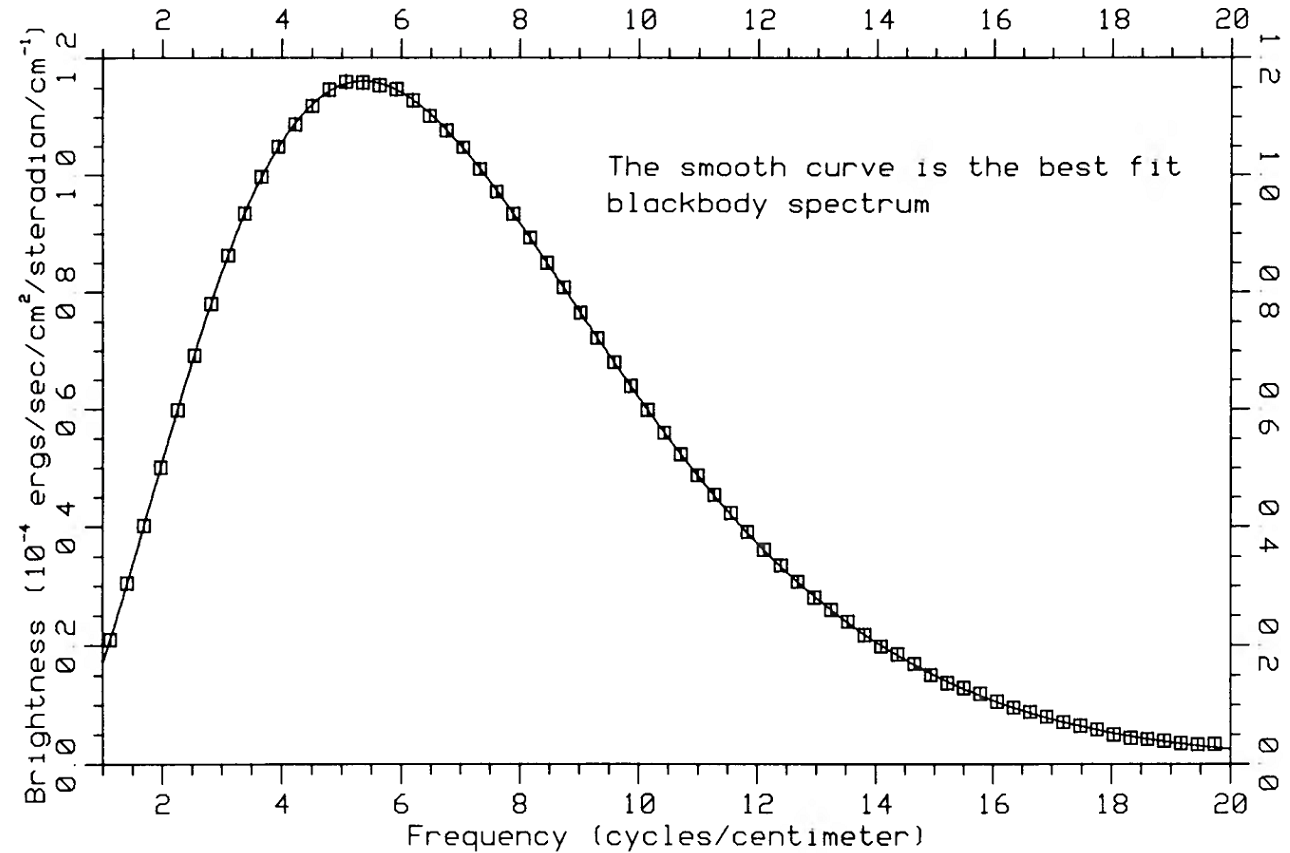
\includegraphics[width=0.7\linewidth]{ScientificMotivation/Figures/FIRAS_CMB_Spectrum_1990.png}
    \caption[FIRAS CMB spectrum (1990)]{Preliminary spectrum of the CMB measured by the FIRAS instrument on the COBE satellite, published in 1990 \cite{mather_preliminary_1990}. The box widths denote the frequency bins for each data point and heights denote a preliminarily stated error bar of 1\%. The error bar of the final spectrum, published in 1994, was orders of magnitude smaller \cite{fixsen_cosmic_1996}.}
    \label{fig:cmb_spectrum}
\end{figure}

In addition to FIRAS, the COBE satellite carried the Differential Microwave Radiometer, which made the first measurement of the CMB isotropy. The spatially mapped intensity fluctuations of the CMB were measured to be one part in ten thousand, demonstrating the extraordinary uniformity of the CMB across the sky. These intensity fluctuations offer a snapshot of the universe $\sim$~370,000 years after the Big Bang, and its hot and cold spots correspond to dark matter over- and under-densities in the primordial plasma. As we will discuss in Section~\ref{sec:anisotropies}, the CMB anisotropies are the seeds of structure formation on which our universe is built.

%%%%%%%%%%%%%%%%%%%%%%%%%%%%%%%%
%%%%%%%%%%%%%%%%%%%%%%%%%%%%%%%%
%%%%%%%%%%%%%%%%%%%%%%%%%%%%%%%%

\section{Inflation}
\label{sec:inflation}

Despite its success, the standard cosmological model fails to explain several outstanding mysteries. Some of these mysteries are at the interface of cosmology and particle physics,  such as $\Lambda$CDM's inability to describe the particle nature of dark matter and dark energy, its inability to describe the matter-antimatter asymmetry, and its predicted baryon abundance that is larger than that directly observed. However, some of the standard cosmological inconsistencies are ``internal,'' in that the assumptions of the model directly contradict the measurements on which it is built. The most prominent of these are...

\begin{itemize}
    \item Horizon problem: the universe appears to have equilibrated across super-horizon length scales, or larger distances than could have ever been in causal contact.
    \item Flatness problem: The universe observed today is very flat, and because any deviation from flatness grows with time, the universe must have begun with a flatness of one part in $\sim$~$10^{14}$, posing a fine-tuning issue.
    \item Magnetic monopole problem: magnetic monopoles are predicted by many grand unified theories, and yet we do not observe any.
    \item Initial conditions: $\Lambda$CDM shows that density perturbations in the early universe evolved into the large-scale structure that we see today. However it does not describe where these initial perturbations come from.
\end{itemize}

There have been several proposed extensions proposed to the Standard Model, but the most popular is \textit{inflation}. The theory of inflation states the universe went through a brief period of exponentially rapid expansion before the Standard Cosmological evolution began.

\begin{figure}[!t]
    \centering
    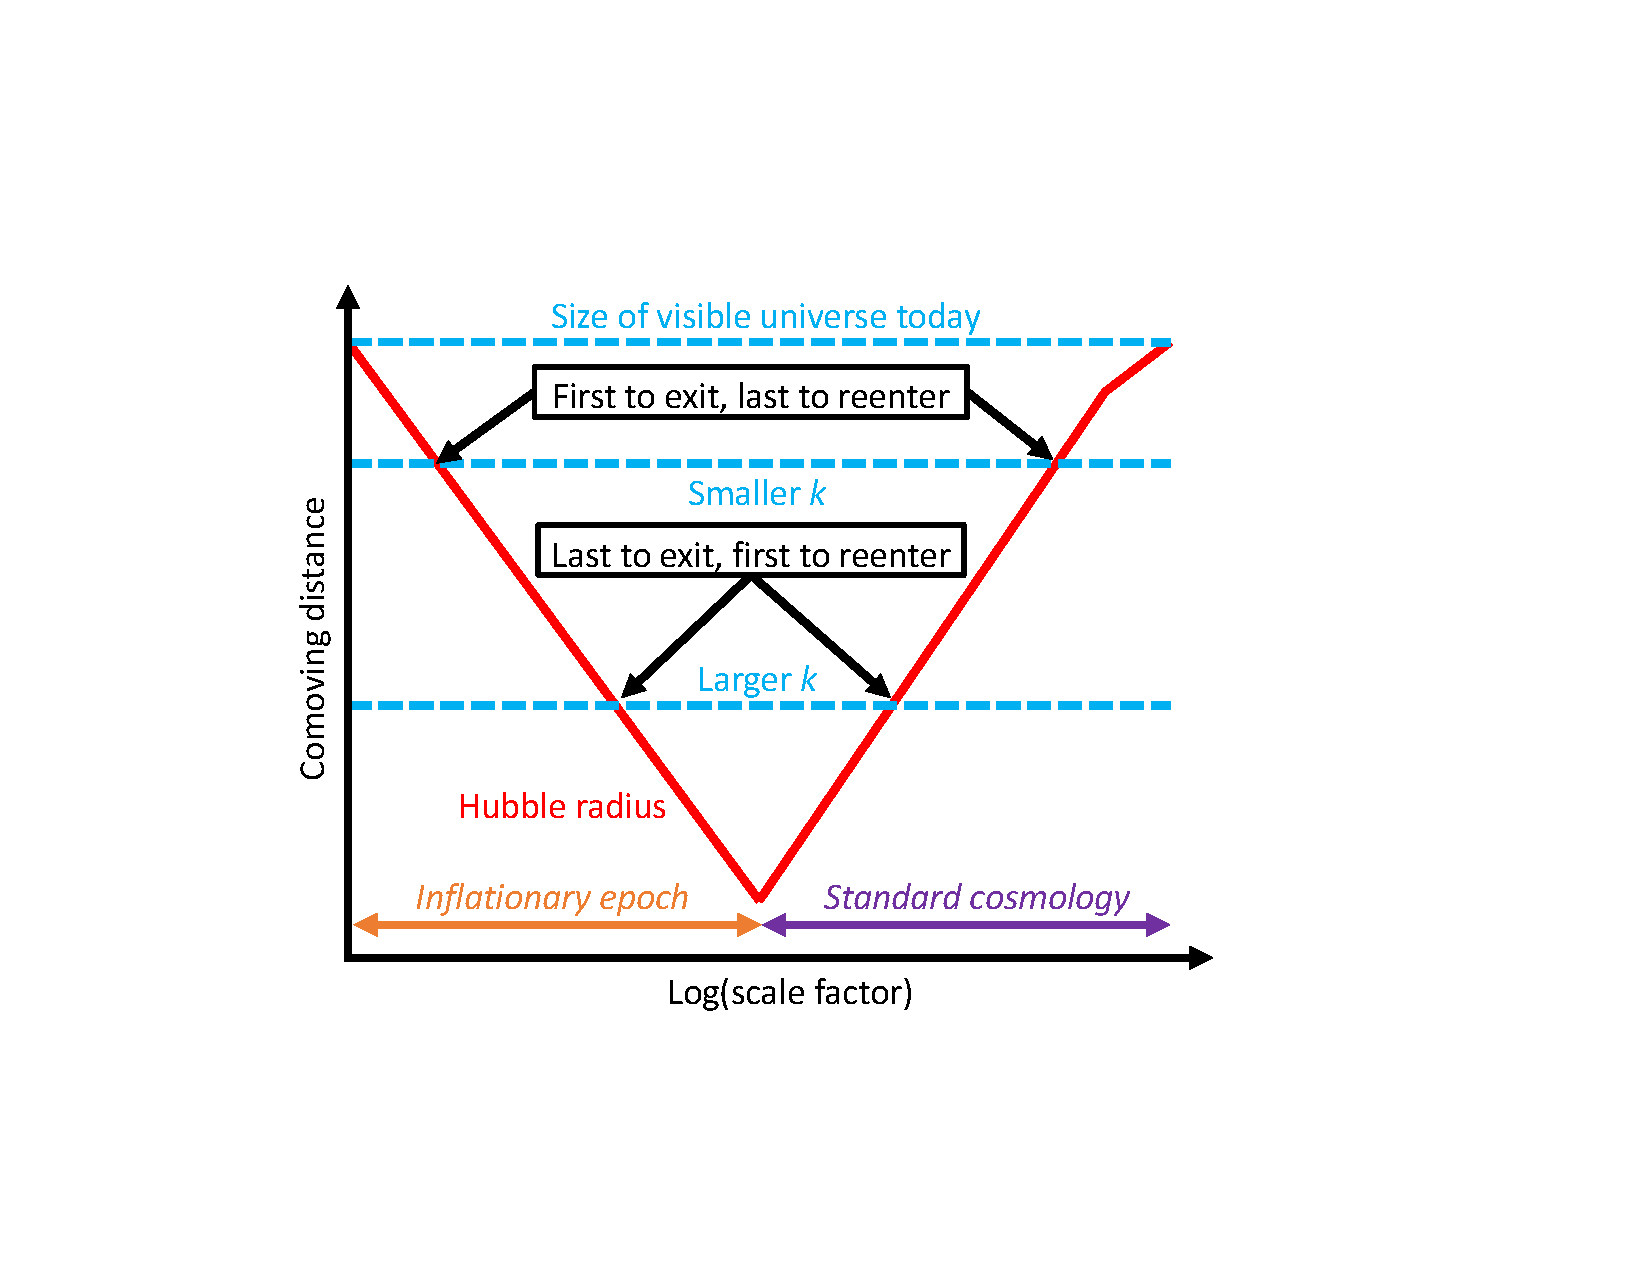
\includegraphics[width=0.6\linewidth, trim=5cm 4cm 7cm 4cm, clip]{ScientificMotivation/Figures/mode_exit_enter.pdf}
    \caption[A figure of mode exit and reentry in in the inflationary paradigm]{A qualitative representation of the relationship between the Hubble Radius---or equivalently the causal horizon---in units of comoving distance vs the scale factor during both the inflationary and standard cosmological epochs. During inflation, the Hubble radius shrinks, freezing length scales that were once in causal contact outside the causal horizon. During the standard cosmological evolution, the Hubble radius grows, and these scales reenter the horizon, allowing them to evolve. The horizontal lines show that small-scale fluctuations exit/enter the horizon first while large-scale fluctuations exit/enter the horizon last. The last scattering surface (LSS) is shown by a blue dotted line, and the kink in the Hubble radius at late times represents the transition from a radiation-dominated universe to a matter-dominated one.}
    \label{fig:mode_entry}
\end{figure}

Figure~\ref{fig:mode_entry} shows a schematic of how the inflationary epoch impacts both spacetime and causal distances. During inflationary expansion, all energy other than that of the inflation field---often called the ``inflaton''---is diluted away, enabling spacetime to expand exponentially.  This exponential expansion is not so different from the accelerating expansion that we witness today, which arises from the dominance of dark energy. Because this exponential expansion enables space to expand faster than the speed of light, the Hubble radius $R_{\mathrm{H}} = 1 / H$, or the length scale that could have at any time been in causal contact, shrinks in comoving coordinates. Note that the $1 / H_{0}$ roughly corresponds to the size of the observable universe today.

The dynamics of the inflationary epoch is governed by the \textit{inflaton}. If we assume that the inflaton is a scalar field $\phi$, as is often the case in the simplest inflationary theories, the Einstein field equations become
\begin{eqnarray}
    & & \ddot{\phi} + 3 H \dot{\phi} + V'[\phi] = 0 \\ 
    & & H^{2} = \frac{\rho_{\phi}}{24 \pi G} \\
    & &\rho_{\phi} = \frac{1}{2} \dot{\phi}^{2} + V[\phi] \, ,
    \label{eq:inflaton}
\end{eqnarray}
where $\phi$ is the inflaton field, $V[\phi]$ is the inflationary potential, and $\rho_{\phi}$ is the inflaton energy density. The first equation, which governs the inflaton's evolution, is nothing more than that of a harmonic oscillator, damped by the Hubble parameter. 

In order to solve the flatness, and horizon problems, the inflaton must follow several \textit{slow-roll} conditions, the dynamics of which are similar to the familiar behavior of a particle in a potential. The slow roll conditions are often given in terms of the \textit{slow-roll parameters}
\begin{equation}
    \epsilon \equiv \frac{m_{\mathrm{pl}}^{2}}{2} \left( \frac{V'[\phi]}{V[\phi]} \right)^{2} \ll 1 \; \; ; \; \; \eta \equiv m_{\mathrm{pl}}^{2} \left| \frac{V''[\phi]}{V[\phi]} \right|, ,
    \label{eq:slow_roll_parameters}
\end{equation}
where $m_{\mathrm{pl}} \equiv \sqrt{\hbar c / G} \sim 10^{19}$~GeV is the Planck mass. These slow roll parameters in turn determine the number of e-folds---or the logarithmic duration---over which inflation occurred
\begin{equation}
    N_{e} = \frac{1}{m_{\mathrm{pl}}} \left| \int_{\phi_{\mathrm{end}}}^{\mathrm{\phi}} \frac{\dd \phi}{\sqrt{2 \epsilon(\phi)}} \right| \simeq 60 - \log{\frac{10^{16} \, \mathrm{GeV}}{V^{1/4}}} \, ,
    \label{eq:efolds}
\end{equation}
where $V$ is the \textit{energy scale of inflation}. As suggested by the approximation in Equation~\ref{eq:efolds}, the number of e-folds needed to resolve the inconsistencies of the standard model is $\sim$~60, which determines, to within an order of magnitude or two, the inflationary energy scale.

\begin{figure}[!t]
    \centering
    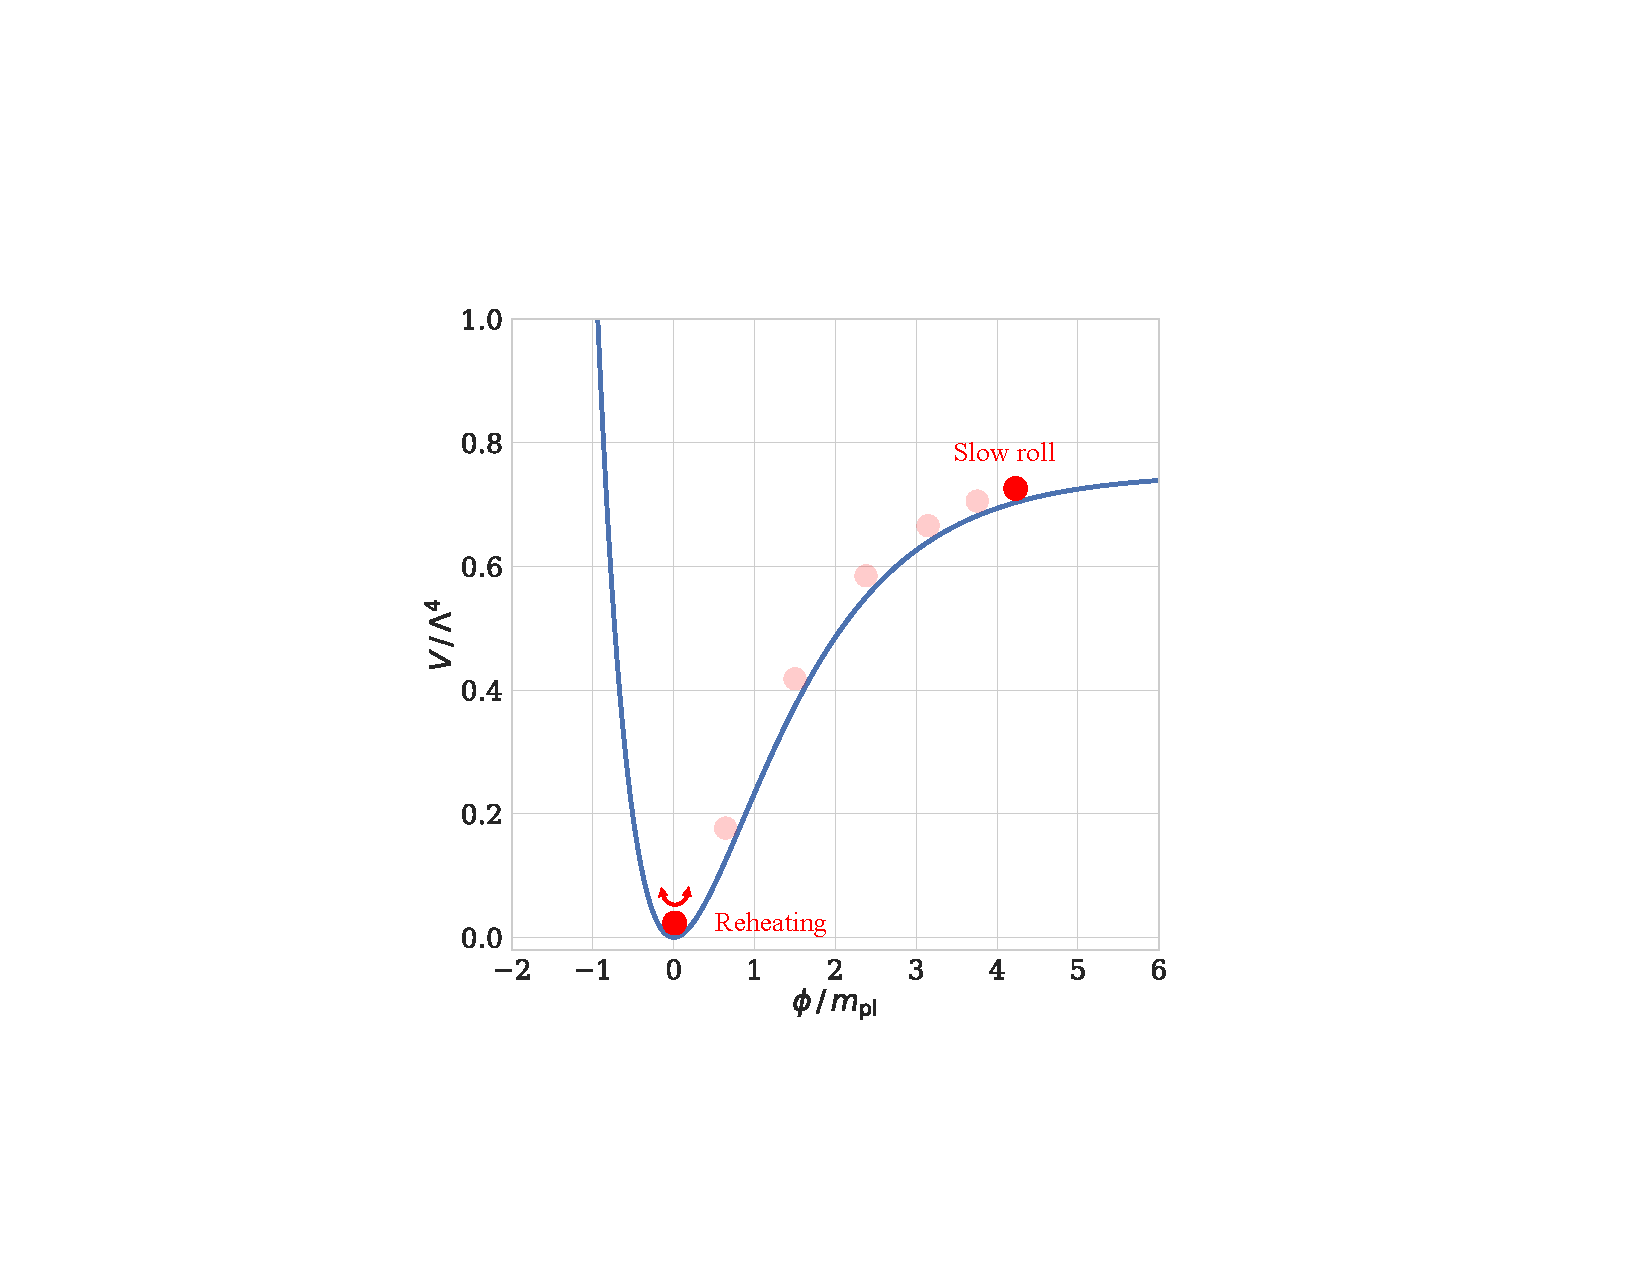
\includegraphics[width=0.7\linewidth, trim=6cm 4cm 6cm 5cm, clip=True]{ScientificMotivation/Figures/inflation_potential.pdf}
    \caption[The $R^{2}$ inflationary potential, which serves as an instructive example of slow-roll inflation.]{}
    \label{fig:inflation_potential}
\end{figure}

As an instructive example, let us consider the potential for Alexei Starobinsky's $R^{2}$ Inflationary Model. This particular model is classified as being \textit{small field} and is derived from a proposed modification to the Einstein-Hilbert action
\begin{equation}
    S = \frac{1}{2 \kappa} \int R \sqrt{| g |} \dd^{4}x \, \rightarrow S_{R^{2}} = \frac{1}{2 \kappa} \int \left(R + \frac{R^{2}}{6 M^{2}} \right) \sqrt{| g |} \dd^{4}x \, ,
    \label{eq:R2_action}
\end{equation}
where $\kappa \equiv 8 \pi G / c^{4}$ is so-called Einstein gravitational constant, $R$ is the Ricci curvature, and $M$ is the model parameter. The potential is found from solving the $R^{2}$ action
\begin{equation}
    V_{R^{2}}[\phi] = \Lambda^{4} \left[ 1 - \exp \left( - \sqrt{2 / 3} \phi / m_{\mathrm{pl}} \right) \right]^{2} \, ,
    \label{eq:starobinsky_potential}
\end{equation}
where $\Lambda$ is the cosmological constant.
The potential is shown in Figure~\ref{fig:inflation_potential} along with a cartoon of the how the inflaton evolves according to Equation~\ref{eq:inflaton}. At $t = 0$, the inflaton is said to be in a ``false vacuum,'' or equivalently an unstable equilibrium. The false vacuum can be constructed in many ways, such as a saddle point, a local minimum in $V[\phi]$, or a flat region, such as for the $R^{2}$ model. At the beginning of inflation, the inflaton \textit{rolls} slowly such that the kinetic term $3 H \dot{\phi} \approx 0$, enabling exponential expansion. However, as the kinetic term grows, both due to an exponentially growing Hubble parameter and due to increasing inflaton evolution, and as the potential term falls near zero, the inflaton decays in a process called \textit{reheating} into the constituents of the standard model. At this point, inflation ends, and the standard cosmological evolution begins.

There are several important outcomes of the inflationary epoch that are compelling within the framework of modern cosmology. First, the the inflationary expansion of spacetime---or equivalently the inflationary contraction of the Hubble radius---allowed the entire observable universe to thermalize prior to $\Lambda$CDM evolution, which solves the horizon problem. Second, the exponential expansion of space would've vastly diluted any spacetime curvatuve that was present at the Big Bang, giving rise to the flat universe we observe today. Third, in a similar manner, the rapid expansion of space would've vastly reduced the density of magnetic monopoles predicted at grand-unified energy scales to a scarcity consistent with their apparent nonexistence today. And finally, quantum fluctuations of the inflation field would have coupled to the metric, in turn seeding the Gaussian-random density variations that we observe in the CMB, hence solving the initial conditions problem.

Despite inflation's elegance and wide popularity, it is not the only proposed extension to the standard model that solves the flatness, horizon, monopole, and intial conditions problems. A prominent competitor is the Ekpyrotic model, which states that the universe is trapped in a never-ending cycle of expanding and collapsing. While Ekpyrosis also solves the horizon, flatness, magnetic monopole, and initial conditions problems, there is one signature that if observed would be a smoking-gun proof that the inflationary paradigm is indeed true: primordial gravitational waves.

Perturbations to the metric are typically classified into three categories: scalar, vector, and tensor. The scalar perturbations arise from density fluctuations, which are sourced by gravity and therefore evolve with underlying dark matter overdensities. Vector perturbations arise from the vortical motions of matter, which are not enhanced by gravity and therefore rapidly die out as the universe expands. Tensor perturbations arise from transverse-traceless perturbations to the metric that propagate by stretching and compressing spacetime, and therefore these tensor perturbation are equivalent to \textit{gravitational waves}. While both inflatin and Ekpyrosis produce Gaussian-random scalar fluctuations, only inflation would have produced a background of primordial gravitational waves.

It is both convenient and powerful to discuss density fluctuations in terms of its power spectrum
\begin{equation}
    \left< \delta(\vec{k}) \delta(\vec{k}') \right> \sim \frac{\delta^{3}(\vec{k} - \vec{k}')}{k^{3}} P(\vec{k})
    \label{eq:density_power_spectrum}
\end{equation}
where the $\sim$ denotes the limit of no mode coupling---enforced by the three-dimensional Dirac delta function---and where $k = | \vec{k} |$. It's worth emphasizing that $k$ is a wavenumber, and therefore large $k$ corresponds to short lengthscales and vice versa. A given mode is able to evolve as long as its wavelength is shorter than the Hubble radius $R_{\mathrm{H}}$, or equivalently when $k \lesssim a H$. As shown in Figure~\ref{fig:mode_entry}, during inflation the Hubble radius rapidly decreases, \textit{freezing out} modes such that they can no longer evolve. In other words, the superluminal expansion of space separates points in space that before inflation were in causal contact. When $k < a H$, the mode can no longer evolve, and it is ``frozen'' until the Hubble radius expands enough for the mode to re-enter the horizon. 

While the Gaussian fluctuations of the inflaton field are thought to be scale independent, the modes exit the horizon from low $k$ to high $k$ as the inflation field $\phi$ rolls down the potential $V[\phi]$, as shown in Figure~\ref{fig:mode_entry}. Therefore, there is a slight tilt in the expected scalar spectrum
\begin{equation}
    P_{\zeta}(k) \equiv A_{\mathrm{s}} \left( \frac{k}{k_{*}} \right)^{n_{\mathrm{s}}(k) - 1} \sim \frac{H_{*}^{2}}{\epsilon_{*} m_{\mathrm{pl}}^{2}} \, ,
    \label{eq:scalar_spctrum}
\end{equation}
where $H_{*}$ and $\epsilon_{*}$ denote the values of the Hubble parameter and the first slow roll parameter, respectively, when the mode $k$ exited the horizon. The spectral tilt is parameterized by the \textit{scalar index}
\begin{equation}
    n_{\mathrm{s}}(k) \equiv 1 + \frac{\dd \log P_{\zeta}(k)}{\dd \log k}
    \, .
    \label{eq:scalar_index}
\end{equation}
In a similar manner, the power spectrum of the tensor perturbations follows the relation
\begin{equation}
    P_{\mathrm{t}}(k) \equiv A_{\mathrm{t}} \left( \frac{k}{k_{*}} \right)^{n_{\mathrm{t}}(k)} \sim \left( \frac{H_{*}}{m_{\mathrm{pl}}} \right)^{2} \, ,
    \label{eq:tensor_spectrum}
\end{equation}
and the tensor index is defined as
\begin{equation}
    n_{\mathrm{t}}(k) \equiv \frac{\dd \log P_{t}(k)}{\dd \log k} \, .
    \label{eq:tensor_index}
\end{equation}
Using these conventions, we expect $n_{\mathrm{s}}$ to be close to 1 and $n_{\mathrm{t}}$ to be close to 0, and we expect each to have a slightly negative slope with $k$. 

The amplitude of the tensor power spectrum is often quoted using the \textit{tensor-to-scalar ratio}
\begin{equation}
    r_{*} \equiv \frac{P_{\mathrm{t}}(k_{*})}{P_{\mathrm{\zeta}}(k_{*})} = \frac{A_{\mathrm{s}}}{A_{\mathrm{t}}} \sim 16 \frac{V_{*}}{A_{\mathrm{s}} m_{\mathrm{P}}^{4}} \, ,
    \label{eq:tensor_to_scalar_ratio}
\end{equation}
where $k_{*}$ is a mode number often chosen by convention by convention to be $k_{*} = 0.05$~$\mathrm{MPc^{-1}}$ and where $V_{*}$ is the inflationay energy scale when mode $k_{*}$ exits the horizon. The tensor-to-scalar ratio can be written in terms of the energy scale of inflation as
\begin{equation}
    V_{*}^{1/4} = 10^{16} \, \mathrm{GeV} \, \left( \frac{r_{*}}{0.01} \right)^{1/4} \, .
    \label{eq:tensor_to_scalar_energy_scale}
\end{equation}
Because the the dependence of the inflationary potential on the tensor to scalar ratio is shallow, a detection of $r_{*}$ would provide a tight constrain $V_{*}$. However, if $V_{*}$ is much lower than the grand unified energy scale $10^{19}$~GeV, then $r_{*}$ may be undetectably small.

%%%%%%%%%%%%%%%%%%%%%%%%%%%%%%%%
%%%%%%%%%%%%%%%%%%%%%%%%%%%%%%%%
%%%%%%%%%%%%%%%%%%%%%%%%%%%%%%%%

\section{CMB anisotropies}
\label{sec:anisotropies}

As discussed in Section~\ref{sec:cmb}, CMB anisotropies trace the underlying dark matter density fluctuations at the time of recombination, and therefore studying their properties illuminates physics of the early universe. The latest full-sky measurement of CMB temperature and polarization anisotropies is from the Planck satellite, and their maps are shown in Figure~\ref{fig:cmb_maps}. 

\begin{figure}[!ht]
    \centering
    \subfloat[\label{fig:cmb_maps:a}]{
        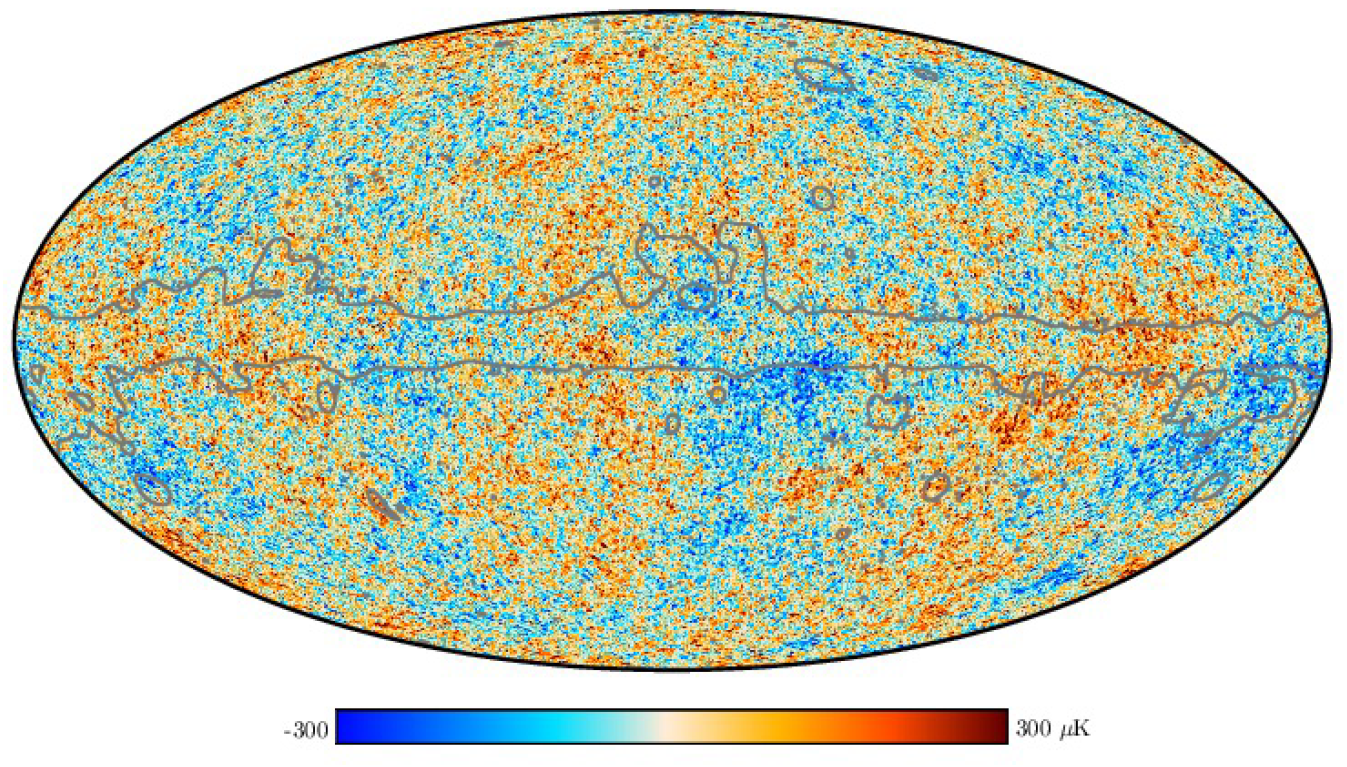
\includegraphics[width=0.7\linewidth]{ScientificMotivation/Figures/Planck_CMB_temperature_2019.png}
    }
    \hfill
    \subfloat[\label{fig:cmb_maps:b}]{
        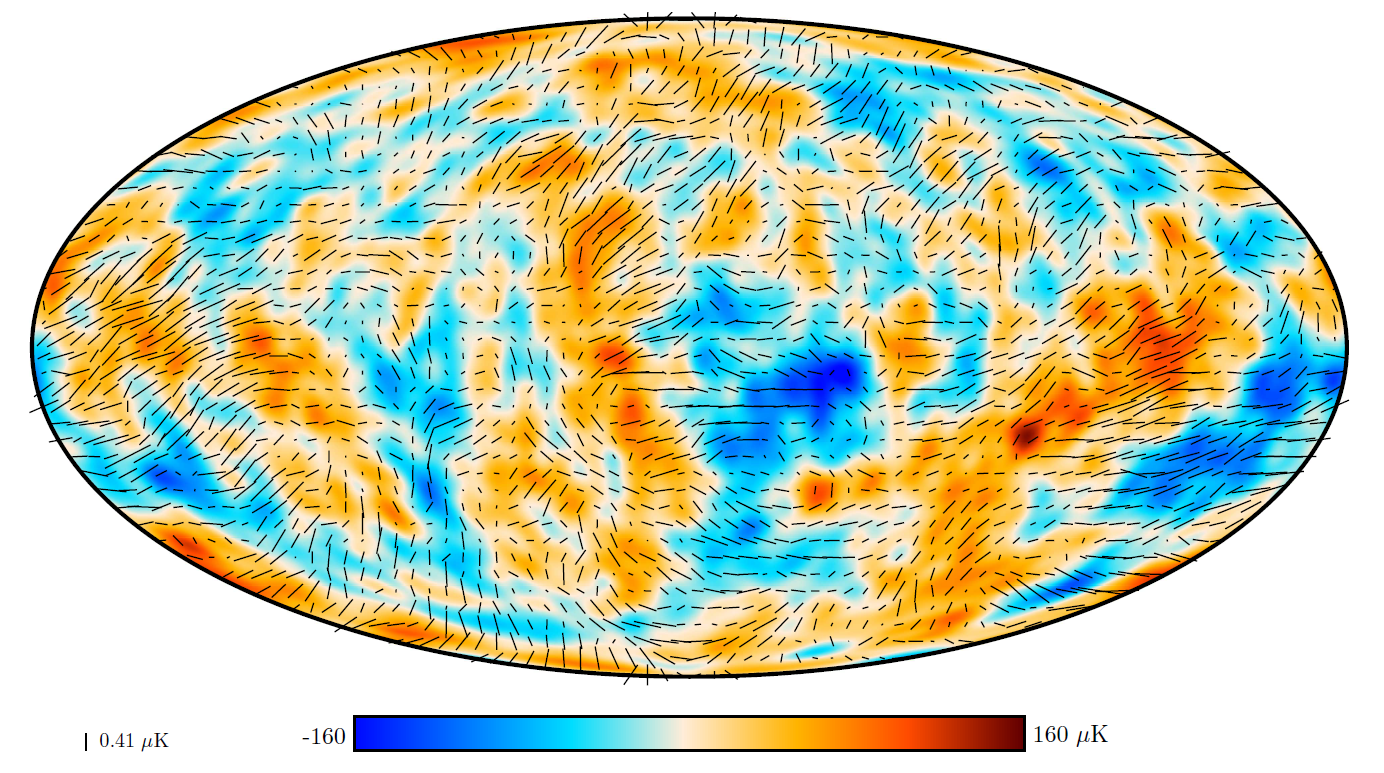
\includegraphics[width=0.7\linewidth]{ScientificMotivation/Figures/Planck_CMB_polarization_2019.png}
    }
    \caption[Planck full-sky CMB temperature and polarization maps (2018)]{Full-sky map of the CMB as presented in the Planck satellite 2018 data release \cite{planck_collaboration_planck_2019}. \ref{fig:cmb_maps:a} shows the temperature anisotropies, with the dominant foreground regions, which are centered around the galactic plane, masked out. \ref{fig:cmb_maps:b} shows the polarization anisotropies smoothed to an angular resolution of 5 degrees for visual clarity.}
    \label{fig:cmb_maps}
\end{figure}

Because the CMB pervades all space and therefore fills the full sky, we can conveniently decompose its temperature fluctuations into spherical harmonics
\begin{equation}
    \Delta T(\hat{n}) = \sum_{\ell = 0}^{\infty} \sum_{m = \ell}^{\ell} a_{\ell m} Y_{\ell m}(\hat{n}) \, ,
    \label{eq:spherical_harmonics}
\end{equation}
where $\hat{n}$ denotes a location on the sky, $(\ell, m)$ are the mode numbers, and $a_{\ell m}$ are the mode amplitudes. As predicted by inflation, the anisotropies of the CMB are isotropic (except the dipole, which arises due to our local motion with respect to the cosmic rest frame) and largely\footnote{As we discuss in Section~\ref{sec:foregrounds}, secondary anisotropies give rise to small levels of non-Gaussianity.} Gaussian, allowing their statistics to be well-described by the temperature power spectrum
\begin{equation}
    \left< \Delta T(\hat{n}) \Delta T(\hat{n}') \right> = \frac{1}{4 \pi} \sum_{\ell = 0}^{\infty} (2 \ell + 1) \, C_{\ell} P_{\ell}(\hat{n} \cdot \hat{n}') \, ,
    \label{eq:temperature_power_spectrum}
\end{equation}
where $P_{\ell}(\cos \theta_{\mathrm{sky}})$ are Legendre Polynomials and the mode variances are defined to be
\begin{equation}
    \left< a_{\ell m} a^{*}_{\ell' m'} \right> = \delta_{\ell m} \delta_{\ell' m'} C_{\ell} \, .
    \label{eq:C_ell}
\end{equation}
$C_{\ell}$ is the variance of the distribution for all $-\ell < m < \ell$ and is a physical measure of the fluctuations for mode $\ell$. Because $\ell = 1$ corresponds to the dipole, the simple relationship 
\begin{equation}
    \theta_{\mathrm{sky}} \sim \frac{180^{\circ}}{\ell} \, ,
    \label{eq:ell_theta_relation}
\end{equation}
relates spherical harmonic mode number to angle on the sky.

For a given $\ell$, there are only $2 \ell + 1$ $m$'s, which means there is a limit to how well one can measure each mode's variance $C_{\ell}$. This limit is called \textit{cosmic variance} and is defined as
\begin{equation}
    \Delta C_{\ell}^{2} = \frac{2}{(2 \ell + 1) f_{\mathrm{sky}}} C_{\ell}^{2} \, ,
    \label{eq:cosmic_variance}
\end{equation}
where $f_{\mathrm{sky}}$ is the fraction of the sky which is measured. The reality of cosmic variance has two important implications for CMB anisotropy measurements. First, because $\Delta C_{\ell} \propto C_{\ell}$, one cannot measure the any given $a_{\ell m}$ distribution with infinite precision, no matter how big the signal is. Second, because larger angular scales have fewer $m$'s, their measurement is more likely to become \textit{cosmic-variance limited}, often motivating larger sky coverage $f_{\mathrm{sky}}$ when measuring low-$\ell$.

\begin{figure}[!t]
    \centering
    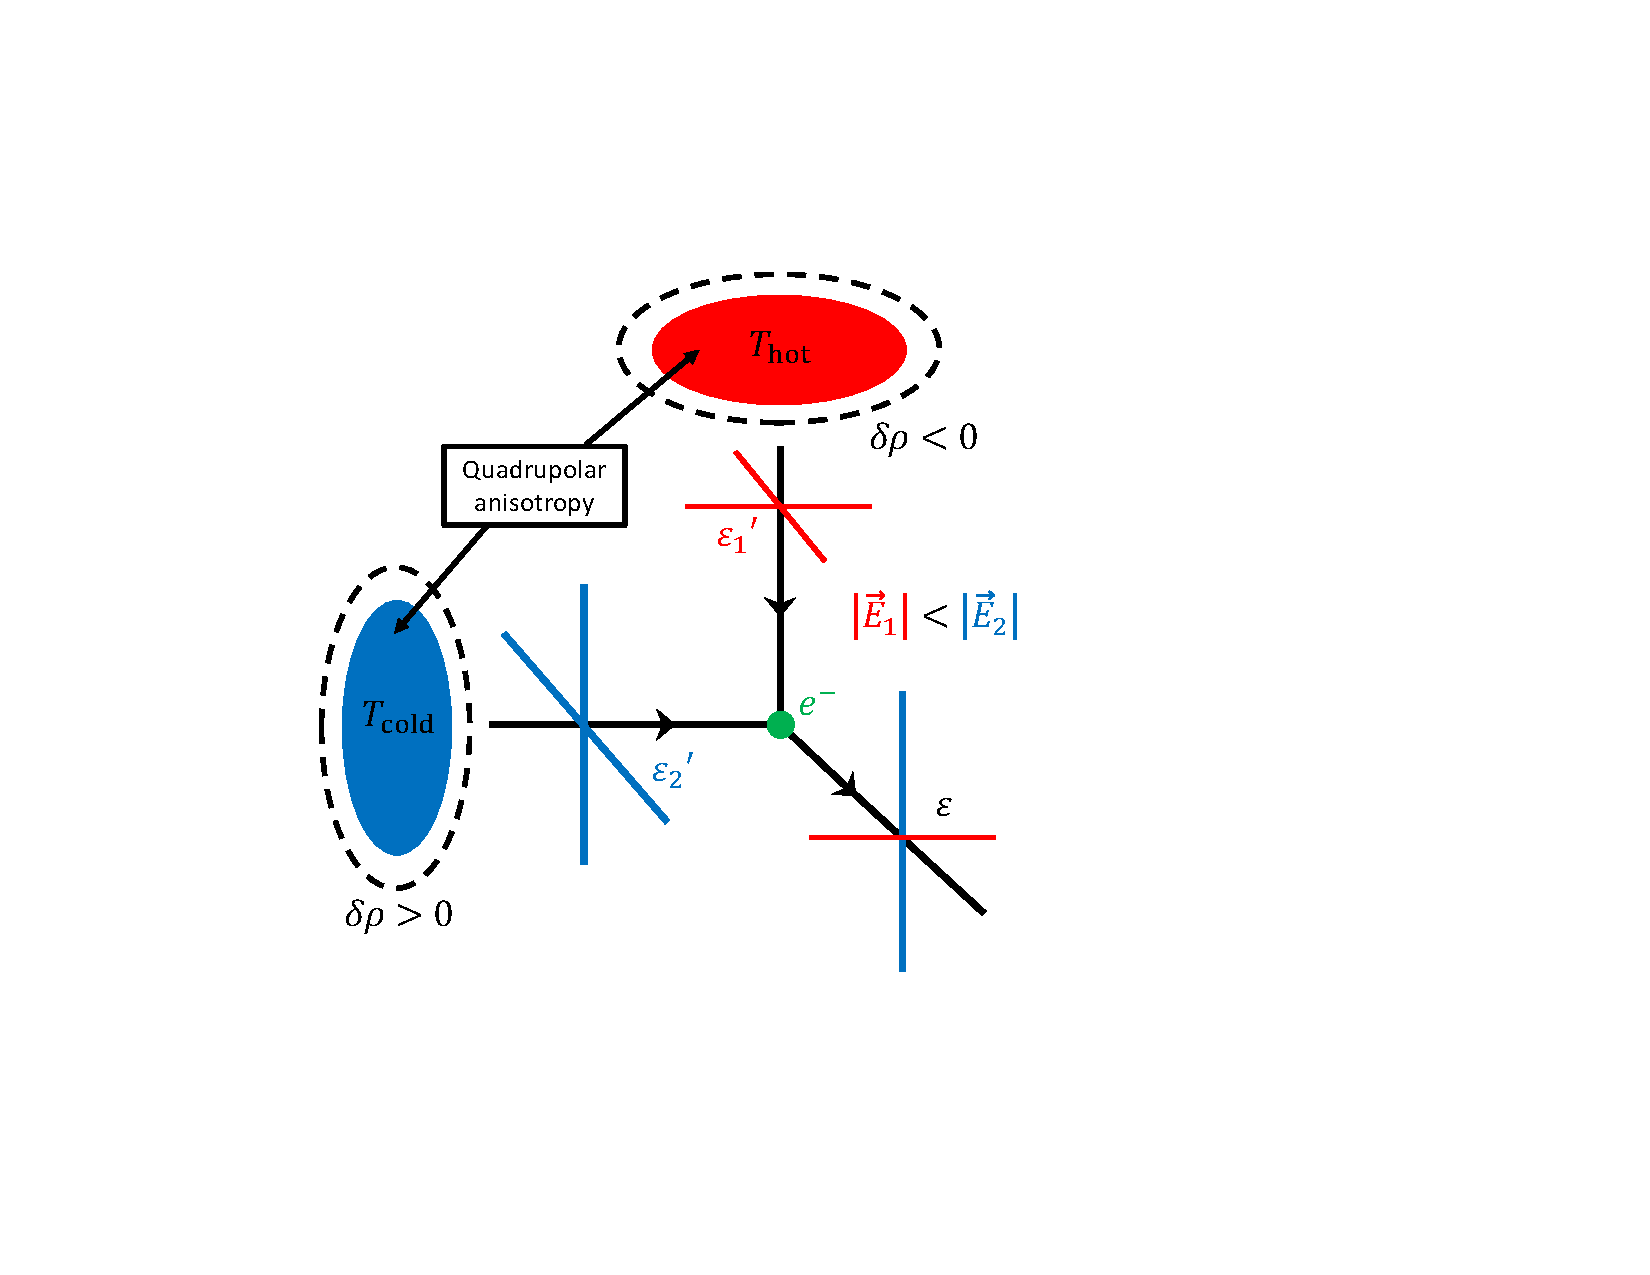
\includegraphics[width=0.5\linewidth, trim=5cm 5cm 10cm 4.5cm, clip]{ScientificMotivation/Figures/thomson_scattering.pdf}
    \caption[Thomson scattering of CMB quadrupolar anisotropies]{A schematic of how temperature anisotropies give rise to linear CMB polarization. Hot/cold spots correspond to gravitational over/underdensities and as photons climb/fall out of these potential wells, they lose/gain momentum $p = h \lambda$, which in turn causes their wavelength to shift down/up. Therefore, ``hot'' photons emerge from \textit{under}densities, while ``cold'' photons emerge from \textit{over}densities. At last scattering, these photons Thomson scatter from a ``taget'' electron $e^{-}$, and when the temperature anisotropy is quadrupolar, the scattered electric fields are not equal $|\vec{E}_{1}| < |\vec{E}_{2}|$, giving rise to a small degree of linear polarization.}
    \label{fig:thomson_scattering}
\end{figure}

In addition to temperature anisotropies, the CMB also contains polarization fluctuations. The CMB is polarized by Thomson scattering of quadrupolar anisotropies at the last scattering surface, as shown in Figure~\ref{fig:thomson_scattering}. The resulting polarization pattern on the sky is often conveniently decomposed into so-called \textit{E-modes} and \textit{B-modes}, which in the \textit{flat-sky approximation} are written as
\begin{eqnarray}
    E(\vec{\ell}) & = & Q(\vec{\ell}) \cos(2 \phi_{\vec{\ell}}) + U(\vec{\ell}) \sin(2 \phi_{\vec{\ell}}) \\
    B(\vec{\ell}) & = & U(\vec{\ell}) \cos(2 \phi_{\vec{\ell}}) - Q(\vec{\ell})\sin(2 \phi_{\vec{\ell}}) \, ,
    \label{eq:emodes_bmodes}
\end{eqnarray}
where $Q = \left< \left| E_{x} \right|^{2} \right> - \left< \left| E_{y} \right|^{2} \right>$ and $U = \left< \left| E_{a} \right|^{2} \right> - \left< \left| E_{b} \right|^{2} \right>$ are the linear-polarization Stokes parameters, $\vec{\ell}$ is the two-dimensional Fourier mode vector, which replaces the ($\ell$, $m$) indices, and $\phi_{\vec{\ell}}$ is the orientation of the mode vector. There are several important properties to notice about the E/B composition. First of all, they are spin-2 fields, meaning that they flip sign under a $\pi/2$ rotation. Secondly, unlike with $Q$ and $U$ explicitly, $E$ and $B$ are not defined with respect to a fixed coordinate system but are instead defined by their symmetry. Figure blah shows an illustration of each basis vector for comparison. E-modes have zero curl and a non-zero divergence, while B-modes have a zero divergence and a non-zero curl. In other words, E-modes have no handedness---or are mirror-symmetric---while B-modes do.

\begin{figure}[!t]
    \centering
    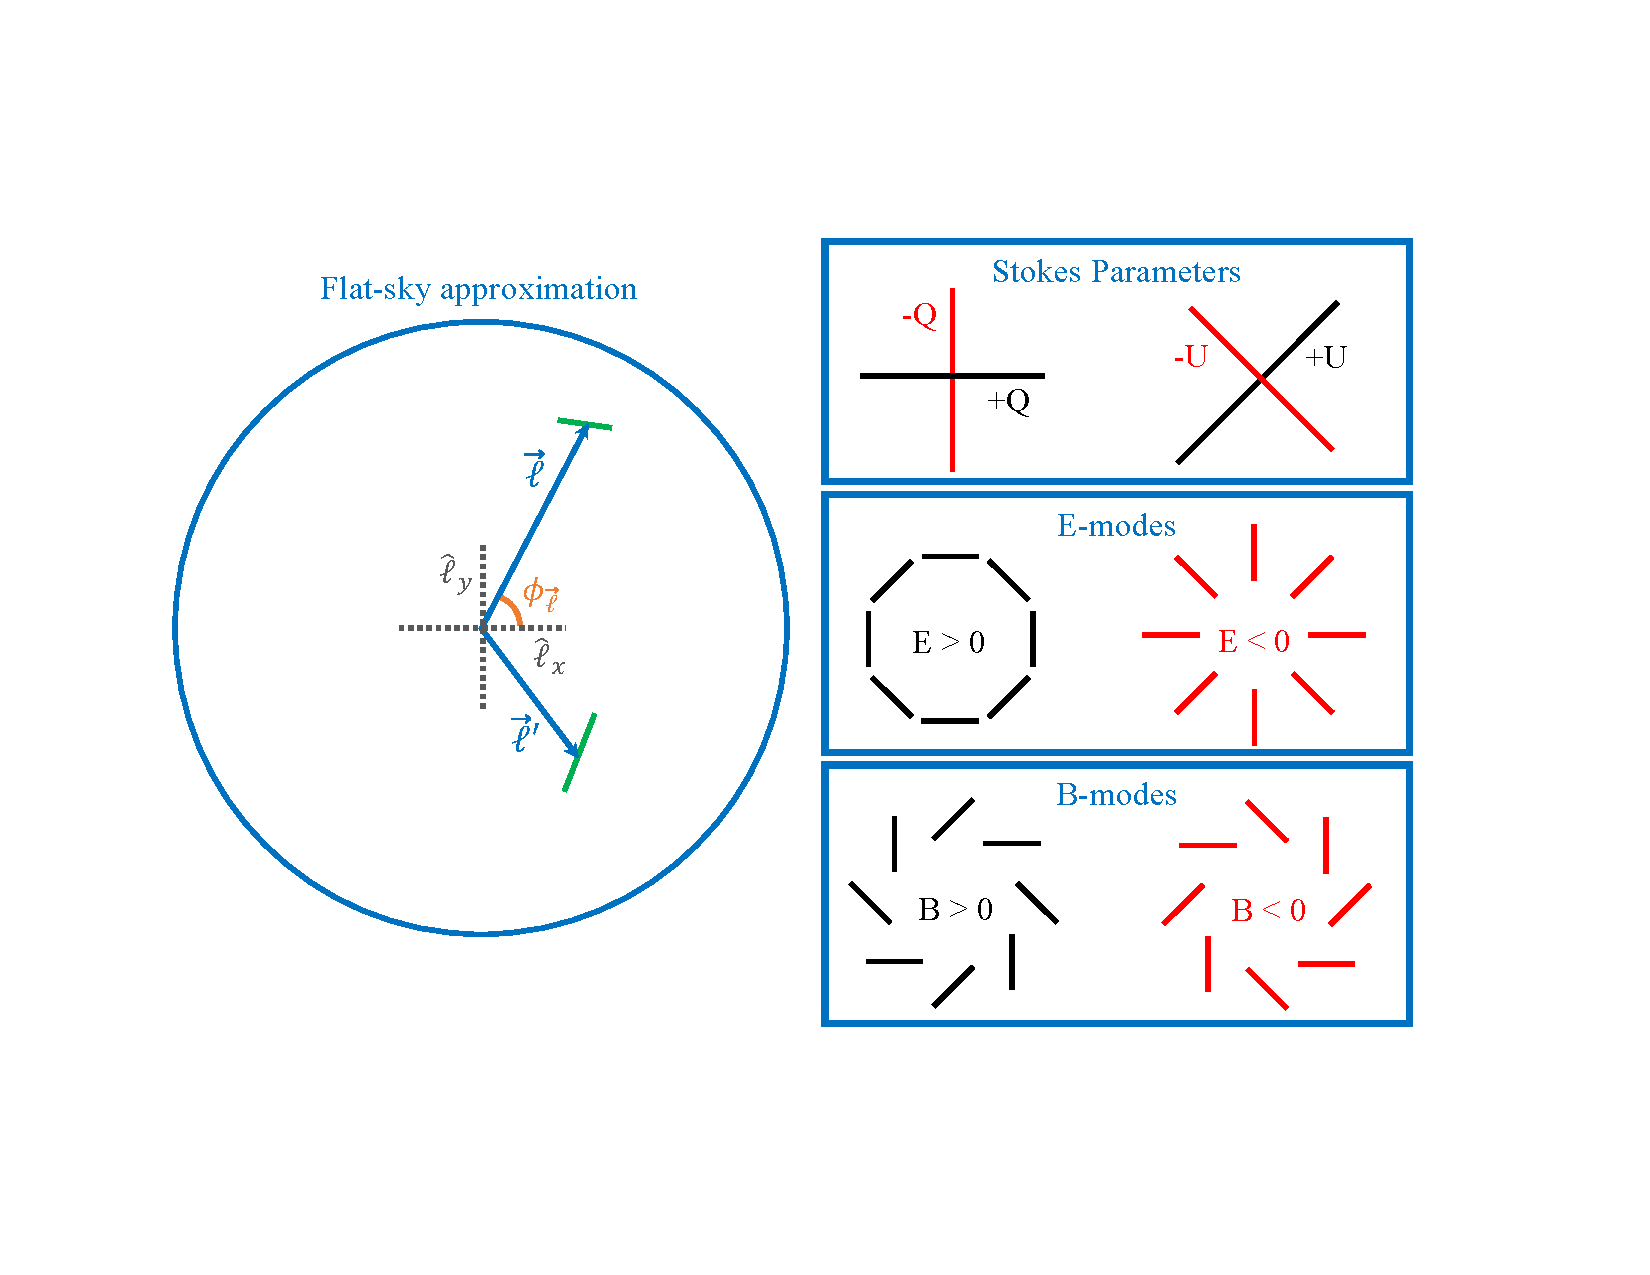
\includegraphics[width=0.8\linewidth, trim=2.5cm 4cm 3.5cm 4cm, clip]{ScientificMotivation/Figures/emodes_bmodes.pdf}
    \caption[Stokes parameters, E-modes, B-modes in the flat-sky approximation]{A schematic of the flat-sky approximation, which quantifies the spherical-harmonic modes using vector $\vec{\ell}$ instead of ($\ell$, $m$). In this scheme, the Stokes vectors Q/U are converted to E-modes and B-modes using Equations~\ref{eq:emodes_bmodes}. As shown in the right panel, E-modes are parity-even, while B-modes are parity-odd. The B-modes' handedness means that they cannot be generated by scalar fluctuations but only by tensor.}
    \label{fig:emodes_bmodes}
\end{figure}

The E-mode/B-mode decomposition is a powerful tool to study the CMB polarization. Because B-modes are only created by tensor perturbations, they are a \textit{null channel} via which primordial gravitational waves can be probed. In other words, a primordial B-mode detection would be a smoking-gun proof of inflation, and such a detection is not limited by cosmic variance (see Equation~\ref{eq:cosmic_variance}).\footnote{In reality, B-mode foregrounds obfuscate the gravitational wave signal, as we will discuss soon} In addition, though only generated by scalar perturbations, E-modes offer their own wealth of information about the univere and its evolution. Just as temperature anisotropies measure the density field of the primordial plasma, E-modes measure the \textit{velocity} field. Additionally, because the CMB is polarized at only the $\sim$~10\% level, the E-mode signal is substantially smaller than that of intensity, allowing for improved cosmic variance in the measurement of both the E-mode variance and the E-mode + temperature correlation. 

%%%%%%%%%%%%%%%%%%%%%%%%%%%%%%%%
%%%%%%%%%%%%%%%%%%%%%%%%%%%%%%%%
%%%%%%%%%%%%%%%%%%%%%%%%%%%%%%%%

\section{CMB power spectrum}
\label{sec:cmb_power_spectrum}

As discussed in Section~\ref{sec:anisotropies}, the fluctuations of the CMB temperature are Gaussian random and are therefore characterized by their variance. This variance depends mode number $\ell$ and is therefore well described by a power spectrum, which measures the amount of fluctuation per angular scale. In spherical-harmonic coordinates, the power spectrum is often written as
\begin{equation}
    D_{\ell}^{XX} = \frac{\ell (\ell + 1) C_{\ell}^{XX}}{2 \pi} \, ,
    \label{eq:D_ell}
\end{equation}
which is chosen for convention because it gives a temperature power spectrum that is roughly flat in $\ell$-space. Here, $XX = (TT, EE, BB, TE, TB, EB)$, noting that we can take various auto and cross spectra between temperature, E-mode, and B-mode fluctuations.

\begin{figure}[!t]
    \centering
    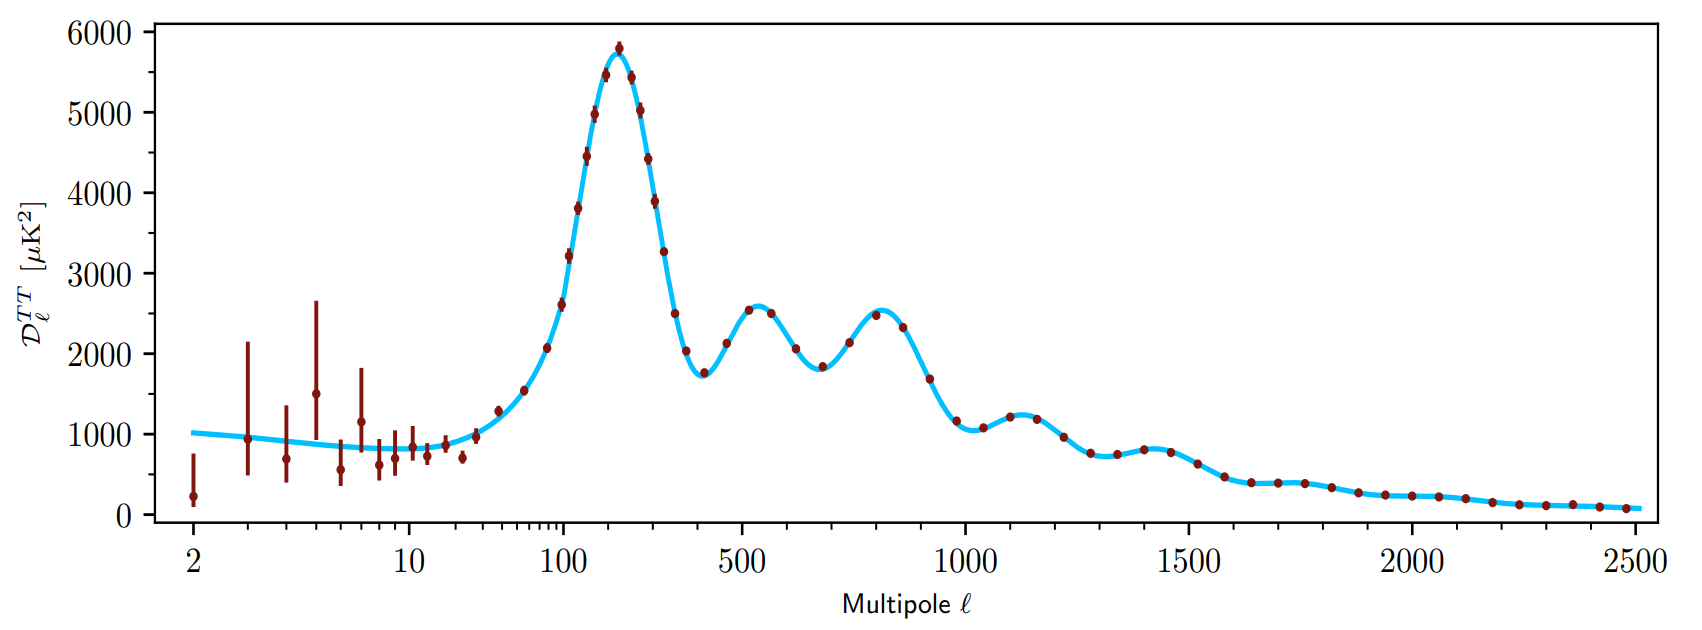
\includegraphics[width=\linewidth]{ScientificMotivation/Figures/Planck_CMB_temperatureSpectrum_2019.png}
    \caption[Planck TT power spectrum]{Autocorrelation power spectrum of the CMB temperature anisotropies as a function of angular scale, as determined using the Planck 2018 data release \cite{planck_collaboration_planck_2019}. The fit corresponds to a $\Lambda$CDM model with six free cosmological parameters: $\Omega_{\mathrm{m}}$, $\Omega_{\mathrm{b}}$, $\theta_{\mathrm{MC}}$, $\tau$, $n_{\mathrm{s}}$, $A_{\mathrm{s}}$. The exquisite precision over a wide range of angular scales is limited by cosmic variance, which fundamentally limits how well we can characterize the statistics of a single realization of the universe.}
    \label{fig:cmb_tt_spectrum}
\end{figure}

The temperature power spectrum, as measured by the Planck satellite, is shown in Figure~\ref{fig:cmb_tt_spectrum}, and it contains several important features that are worth noting. Mirroring the discussion in Section~\ref{sec:inflation}, we move from low-$\ell$ to high-$\ell$, which corresponds to the first/last modes to exit/enter the horizon in Figure~\ref{fig:mode_entry}. At $\ell \lesssim 100$, or on angular scales $\theta_{\mathrm{sky}} \lesssim 1^{\circ}$, the spectrum is nearly flat. These modes exist outside of the horizon at the time of last scattering and therefore have not evolved since they exited the horizon during the inflationary epoch. In principle, these low-$\ell$ modes could be used to measure $r$, as gravitational waves give rise to temperature fluctuations. However, $D_{\ell}^{TT}$ is dominated by gravitational redshifting at the surface of last scattering, also called the \textit{Sachs-Wolfe Effect}, and the measurement precision is limited by cosmic variance.

Moving to higher-$\ell$, there is a series of peaks which are generated by baryon acoustic oscillations (BAOs). Because these modes are of a shorter length scale, they enter the horizon before recombination and therefore evolved according to the physics of the primordial plasma. BAOs are acoustic waves that arise from compression due to gravitational dark matter overdensities and rarefaction due to photon pressure in the primordial fluid. The peaks in the spectrum correspond to the scales at which the oscillations are at maximum rarefaction (odd peaks) and maximum compression (even peaks). When the CMB decoupled, the baryonic matter was frozen into place, and their remnant was imprinted onto the CMB anisotropies. As the universe continues to evolve after recombination, the underlying dark matter densities cause the baryons to accumulate, leading to the formation of structure that we observe today. At $\ell \gtrsim 1000$ the BAO peaks are suppressed by \textit{Silk damping}, which arises when the length scale of the BAOs is shorter than the photon diffusion length. The impact of Silk damping is heightened by the finite duration of recombination, when the universe phase transitions from opaque to quite transparent. During the recombination epoch, the photon diffusion length increases rapidly, pushing the Silk damping tail to lower $\ell$ than if recombination had been instantaneous. 

As is evident in Figure~\ref{fig:cmb_spectrum}, the measurement of the temperature power spectrum is exquisite. The Planck satellite measured the full spectrum to nearly cosmic variance, and the data is described to very high prevision by $\Lambda$CDM. In addition, a plethora of experiments have independently verified the shown $TT$ spectrum across a range of $\ell$ from 2~$\sim$~5000 (above this scale, the measured temperature power spectrum becomes dominated by unresolved point sources, which are difficult to remove).

\begin{figure}[!t]
    \subfloat[\label{fig:cmb_ee_bb_spectrum:a}]{
        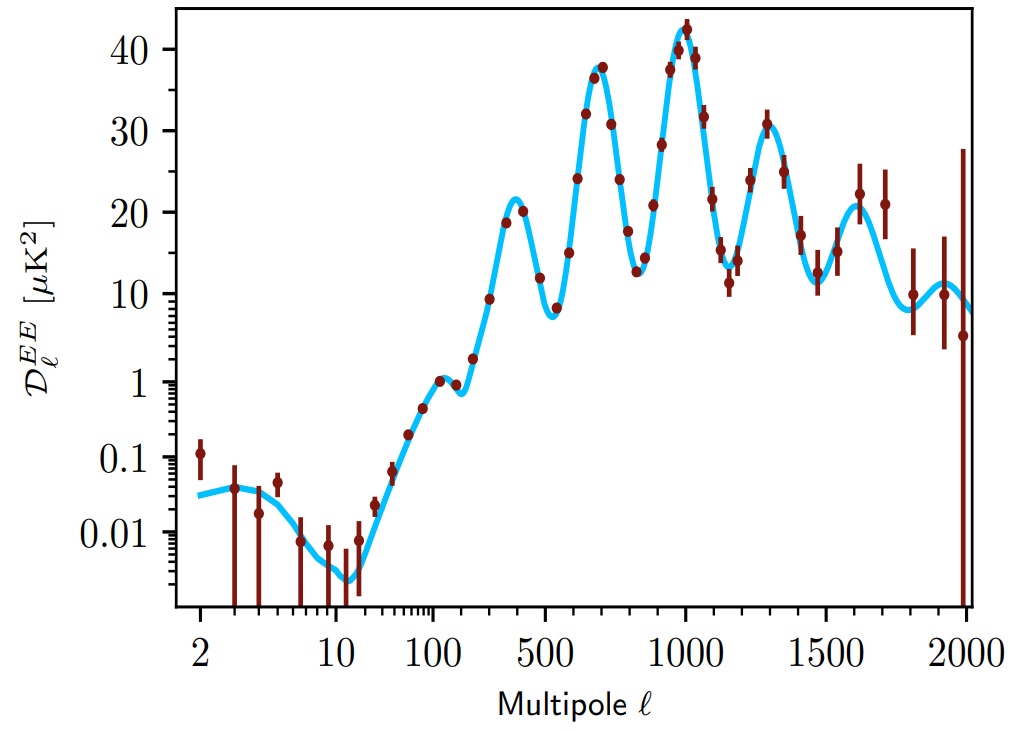
\includegraphics[width=0.6\linewidth, trim=0cm 0cm 0cm 0cm, clip]{ScientificMotivation/Figures/Planck_CMB_EEspectrum_2019.png}}
    \subfloat[\label{fig:cmb_ee_bb_spectrum:b}]{
        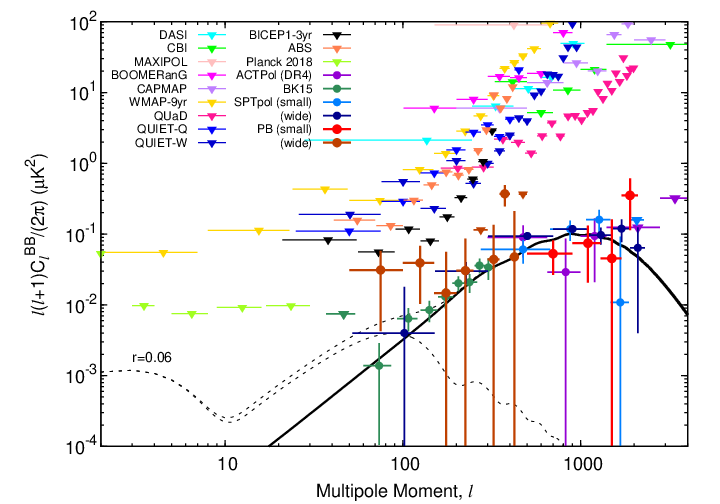
\includegraphics[width=0.6\linewidth, trim=0cm 0cm 0cm 0cm, clip]{ScientificMotivation/Figures/bb_yuji.png}}
    \caption{Power spectrum of the CMB E-mode anisotropies as measured by Planck (top panel) and B-mode anisotropies as measrued by several experiments. The $EE$ features are due to the velocity field of BAO and its fit uses the same cosmological parameters as that of Figure~\ref{fig:cmb_tt_spectrum}, while the B-mode spectrum arises due to gravitational lensing of the E-modes. The dotted lines represent the current 95\% upper limits on the primordial B-mode spectrum.}
    \label{fig:cmb_ee_bb_spectrum}
\end{figure}

CMB polarization measurements have just recently begun to come into focus. The EE spectrum, shown in the top panel of Figure~\ref{fig:cmb_ee_bb_spectrum}, is also generated by BAO but is the result of photon velocities, which create redshifts that when quadrupolar about the scattering electron, creating polarization via Thomson Scattering. Because quadrupolar BAO fluctuations are are less prominent than those of the monopole, the CMB's polarization fraction $\lesssim$~10\%, and the $EE$ spectrum is orders of magnitude below that of $TT$. Additionally, though both generated by BAO, the velocity-generated $EE$ peaks are out of phase with the density-generated $TT$ peaks. At $\ell \gtrsim 1500$, photon diffusion damps the $EE$ spectrum similarly to $TT$, but at low-$\ell$, the physics of temperature an polarization anisotropies are distinct. Because there is no polarization analog to the Sachs-Wolfe Effect, the the polarization spectrum at 10~$<$~$\ell$~$<$~100 has a slope of $\ell (\ell + 1)$, corresponding to a scale-independent variance $C_{\ell}^{EE}$. On very large scales $\ell$~$<$~10, there is an excess anisotropy which corresponds to modes that reentered after the epoch of \textit{reionization}, which is when the interstellar medium is ionized by radiation from stars. CMB photons recouple to this interstellar plasma and late-time dark matter fluctuations, and this in turn generates additional Thomson scattering. The height of this peak  $\tau$  

The primordial BB spectrum is only present if primordial gravitational waves are generated by inflation. The polarization mechanism is similar to that of the E-modes, except instead of acoustic oscillations generating the photon redshifts, it is the distortion of the underlying metric by gravitational waves. Because tensor modes are not enhanced by gravitational structure, such as is true for acoustic oscillations, they are quickly washed out after reentering the horizon. Therefore, the primordial $BB$ peak is theorized to be at $\ell \sim 100$, above which it rapidly decreases. This reality makes a measurement of $n_{\mathrm{t}}$ an extraordinary challenge, especially in the presence of gravitationally lensed B-modes.

%%%%%%%%%%%%%%%%%%%%%%%%%%%%%%%%
%%%%%%%%%%%%%%%%%%%%%%%%%%%%%%%%
%%%%%%%%%%%%%%%%%%%%%%%%%%%%%%%%

\section{Foregrounds}
\label{sec:foregrounds}

As mentioned in Section~\ref{sec:cmb_power_spectrum}, the BB spectrum, while in theory a null probe of tensor modes, is in reality obfuscated by foregrounds. An accurate characterization and removal of these foregrounds is becoming increasingly central to an effective primordial B-mode measurement.

The first B-mode foreground is that of gravitational lensing. After last scattering, photons stream freely, but their paths are altered by intervening gravitational structure, as dark matter distorts the underling metric (as in Equation~\ref{eq:einstein_field_equation}). When viewing the CMB, these deflections distort the temperature and polarization maps, inducing non-Gaussian affects that includes the coupling of E-modes and B-modes. The spectrum of these \textit{lensing B-modes} is the convolution of the line-of-sight gravitational potential and the E-mode power, and its spectrum peaks at a similar angular scale to that of the E-modes, at $\ell \sim 1000$. When $\ell \gtrsim 200$, the lensing B-mode power is larger than the B-mode power for $r \sim 0.1$, making a measurement of the tensor spectral index $n_{\mathrm{t}}$ extraordinarily challenging in any circumstance. When $r \lesssim 0.01$, lensing B-modes swamp primordial B-modes for all $\ell \gtrsim 50$, necessitating a process called \textit{delensing} to reveal the primoridal B-mode signal. While still in its infancy, removing 90+\% of lensing power is an extraordinary challenge and is pushing CMB observatories to measure a wide range of angular scales $\ell$~10~$\sim$~1000.

It's worth noting that at very low-$\ell$, there is another peak in B-mode power which is not buried by lensing B-mode power. This peak is due to reionization---an epoch at $z \sim 6$ when diffuse neutral hydrogen once again ionizes due to ultraviolet radiation from stars---and offers an alternative to delensing. Measuring such larger angular scales from the ground is very difficult (see Section HWP for a detailed discussion), and even in the event of a prefect measurement, its precision will be limited by cosmic variance. Nonetheless, the reionization peak is one of the most promising avenues to measure primordial B-modes and is the target of the Cosmology Large Angular Scale Surveyor (CLASS) experiment and future satellite experiments, such as LiteBIRD. 

The second foreground contaminant to primordial B-modes is that of the Milky Way. The interstellar medium (ISM) is filled with dust, which is a complex composition of tiny grains that absorb and emit thermal radiation. While the dust is concentrated around the galactic plane, it is bright enough to contaminate even the cleanest portions of the sky. In addition, the ISM is filled with synchrotron radiation, generated by relativistic charged particles whirling through the galaxy's magnetic field. While the galactic magnetic field isn't presently well understood, it is known to have coherent structure, and synchrotron radiation is known to be highly polarized. 

Dust and synchrotron is 

\begin{figure}[!ht]
    \subfloat[\label{fig:cmb_ee_spectrum:a}]{
        \raisebox{0.6cm}{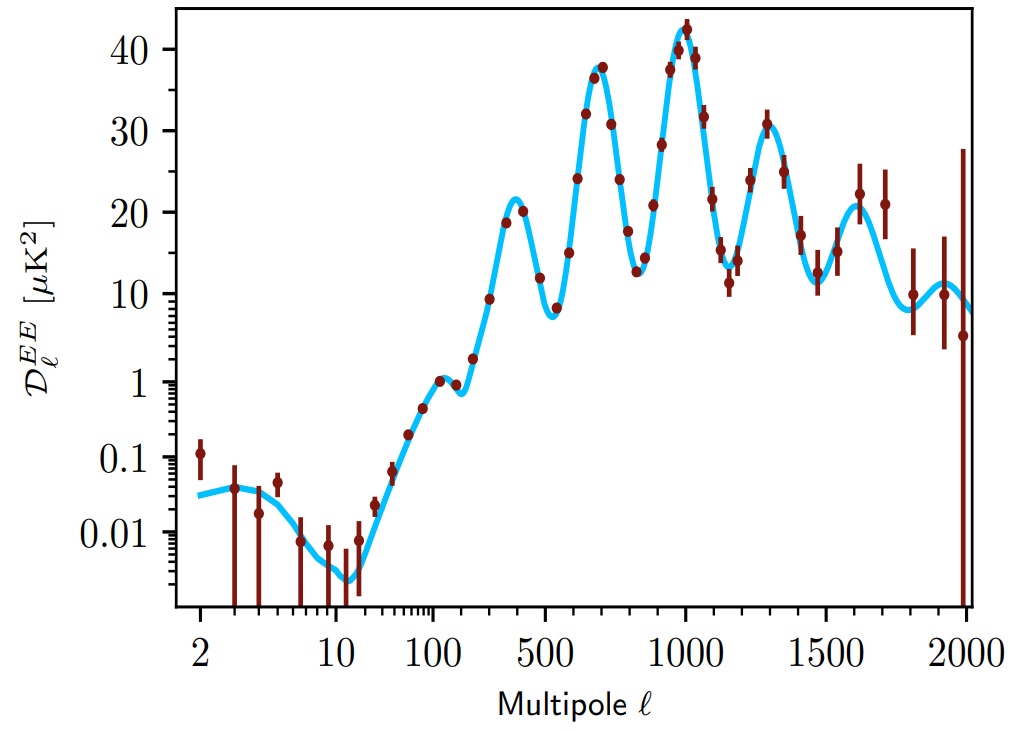
\includegraphics[width=0.45\linewidth]{ScientificMotivation/Figures/Planck_CMB_EEspectrum_2019.png}}
    }
    \hfill
    \subfloat[\label{fig:cmb_ee_spectrum:b}]{
        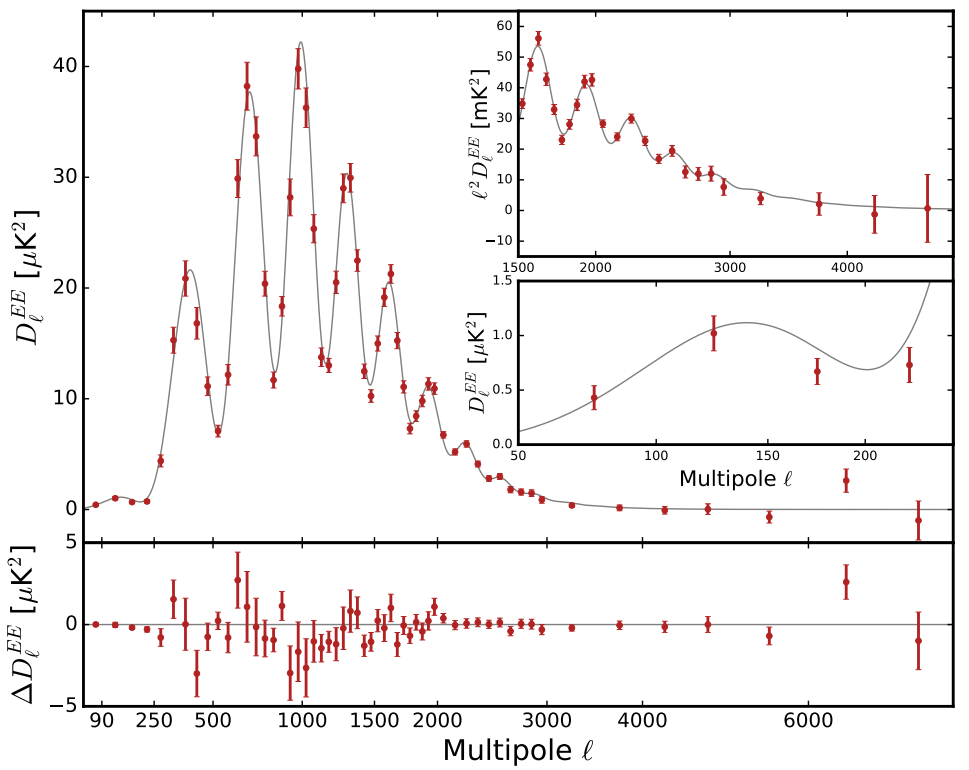
\includegraphics[width=0.51\linewidth]{ScientificMotivation/Figures/SPT_CMB_EEspectrum_2018.png}
    }
    \caption[Planck and SPT EE power spectra]{Autocorrelation power spectra of the CMB E-mode anisotropies as a function of angular scale. \ref{fig:cmb_ee_spectrum:a} shows the EE measurement presented in the Planck 2018 data release and shows exquisite agreement with the best-fit $\Lambda$CDM model to $\ell \sim 1500$ \cite{planck_collaboration_planck_2019}. \ref{fig:cmb_ee_spectrum:b} shows the EE measurement presented by the SPT collaboration in 2018, agreeing closely with the Planck spectrum at low-$\ell$ while also fitting the model well out to smaller angular scales.}
    \label{fig:cmb_ee_spectrum}
\end{figure}

\begin{figure}
    \centering
    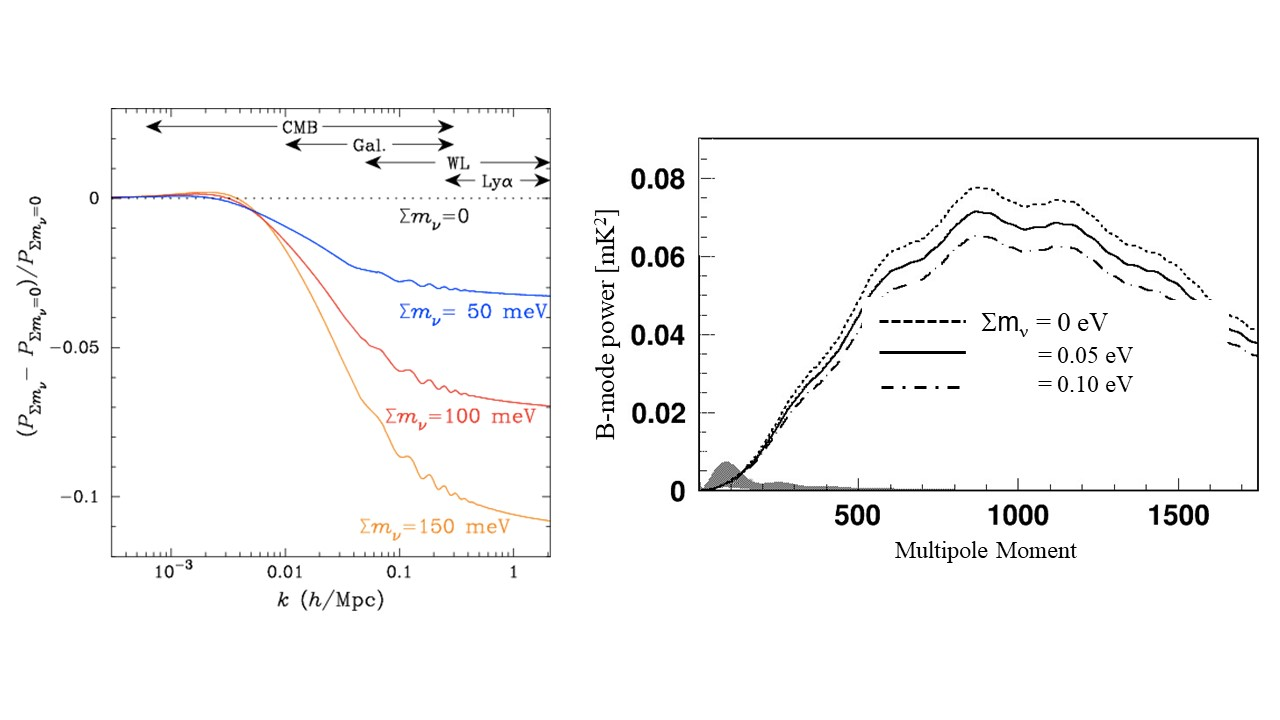
\includegraphics[width=\linewidth, trim=0cm 2cm 0cm 2cm, clip]{ScientificMotivation/Figures/neutrino_ps.jpg}
    \caption[Effect of cosmic neutrinos on the matter and CMB B-mode power spectra]{Effect of cosmic neutrinos on the matter and CMB B-mode power spectra. The figure on the left shows the fractional suppression in matter power vs neutrino mass, compared to the hypothetical case of no neutrinos. The degree of suppression is governed by the fraction of matter that sreams freely and hence smears structure on small scales. The figure on the right shows the impact of cosmic neutrinos on the CMB B-mode power spectrum. The structure suppression at these earlier times is governed by the point at which the neutrinos transition from relativistic to non-relativistic particles, which in turn impacts the physics of the early-time Integrated Sachs-Wolfe effect. The larger the neutrino mass, the earlier the universe transitions from radiation-dominated to matter-dominated, and hence the less strucutre seen in the CMB. \cite{abazajian_neutrino_2015}}
    \label{fig:neutrino_ps}
\end{figure}

\begin{figure}[!ht]
    \subfloat[\label{fig:foreground_spectra:a}]{
        \raisebox{0.5cm}{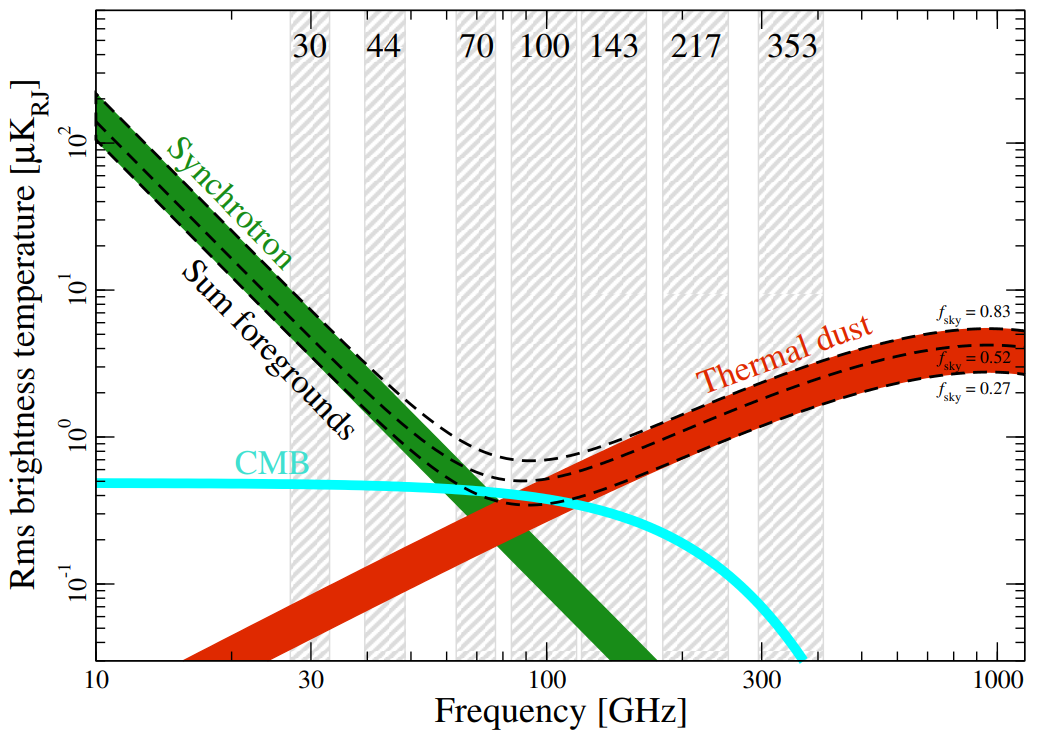
\includegraphics[width=0.45\linewidth]{ScientificMotivation/Figures/Foreground_spectrum_Planck_2019.png}}
    }
    \hfill
    \subfloat[\label{fig:foreground_spectra:b}]{
        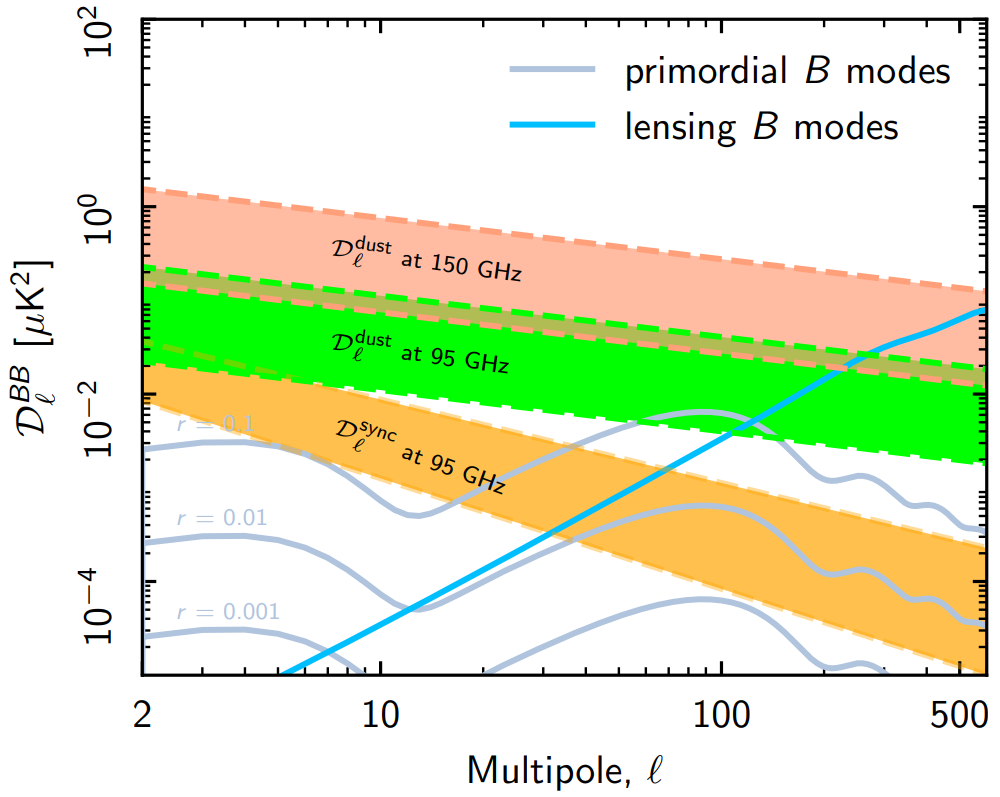
\includegraphics[width=0.45\linewidth]{ScientificMotivation/Figures/Foreground_angularSpectrum_Planck_2019.png}
    }
    \caption[Polarized foreground frequency and angular power spectra]{The intensity of polarized synchrotron and dust compared to that of the CMB. \ref{fig:foreground_spectra:a} shows spatially averaged foreground brightness vs frequency for various fractions of the sky \cite{planck_collaboration_planck_2019}. \ref{fig:foreground_spectra:b} shows the angular power spectrum of dust and synchrotron at two common CMB observation frequencies, compared to the lensing B-mode spectrum and a possible primordial B-mode spectra \cite{planck_collaboration_planck_2018}.}
    \label{fig:foreground_spectra}
\end{figure}

\section{State of the field}

\begin{figure}[!ht]
    \subfloat[\label{fig:bb_spectrum:a}]{
        \raisebox{1.1cm}{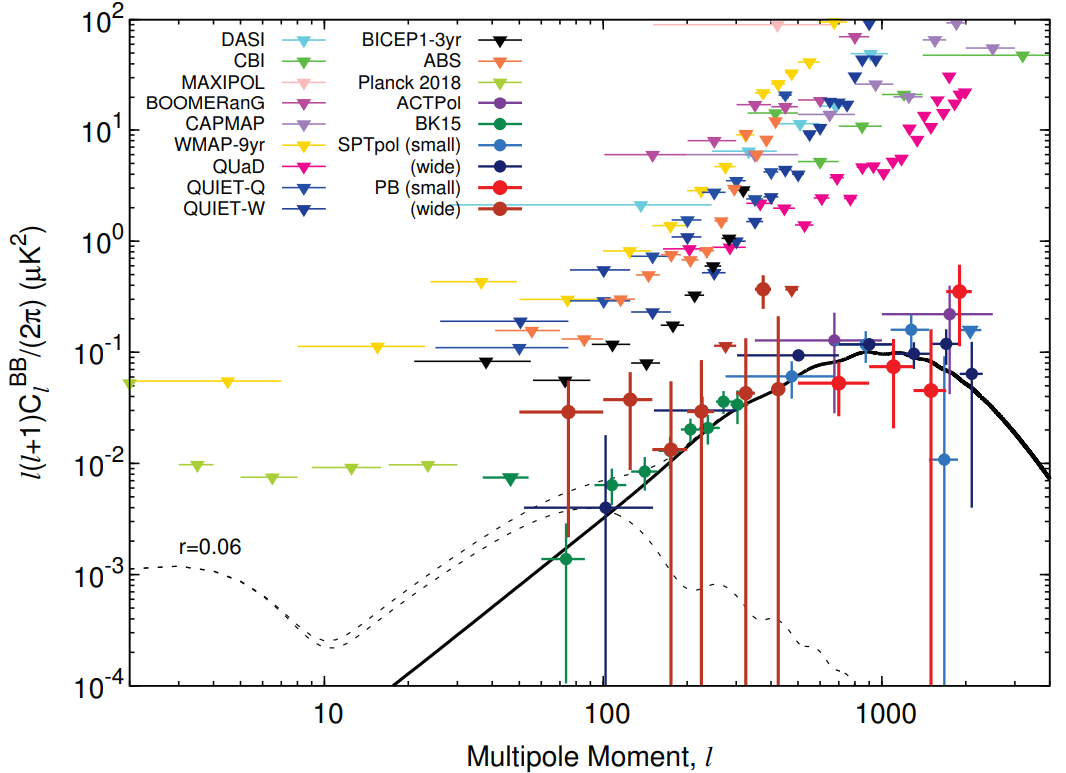
\includegraphics[width=0.45\linewidth]{ScientificMotivation/Figures/Yuji_BB_spectrum.png}}
    }
    \hfill
    \subfloat[\label{fig:bb_spectrum:b}]{
        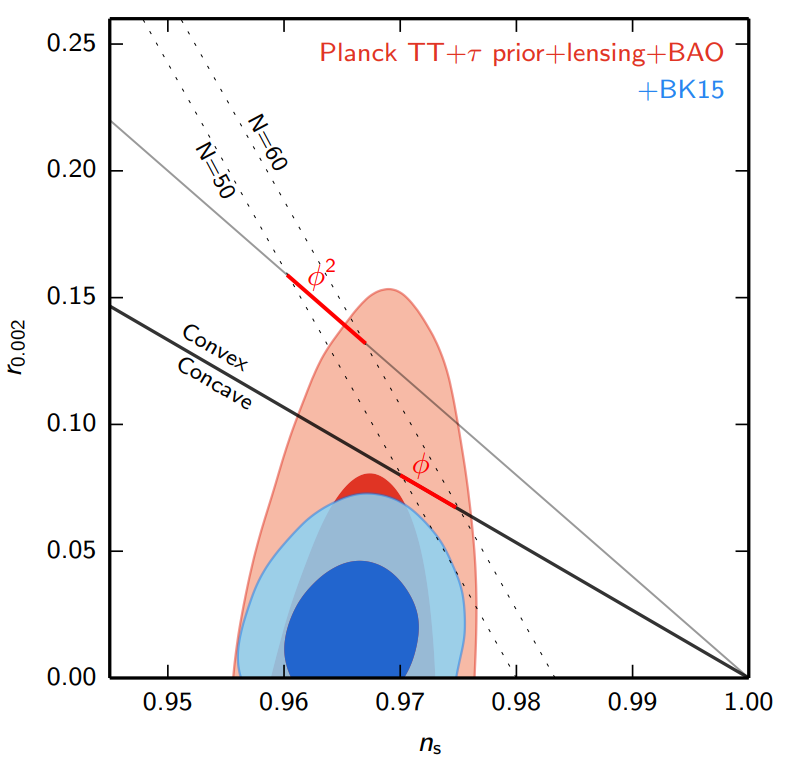
\includegraphics[width=0.45\linewidth]{ScientificMotivation/Figures/Keck_r_ns_2018.png}
    }
    \caption[Current state of the BB measurement and exclusion regions in the r vs $n_{\mathrm{s}}$ plane]{The current state of the CMB B-mode polarization autocorrelation power spectrum, as well as it implications for constraints on inflation. \ref{fig:bb_spectrum:a} shows the history of B-mode measurements made by various experiments. The triangles represent upper limits, and the circles and crosses represent central values and uncertainties, respectively. The solid line is the best-fit, foreground-subtracted lensing spectrum as determined by the latest BICEP/Keck result, and the dotted line represents the current upper bound on $r$, which parameterizes primordial gravitational waves. Figure courtesy of Dr. Yuji Chinone. \ref{fig:bb_spectrum:b} shows the exclusion contours in the $r$-$n_{\mathrm{s}}$ plane when combining data from BAO, Planck, and BICEP/Keck \cite{array_bicep2_2018}.}
    \label{fig:bb_spectrum}
\end{figure}
